\documentclass[twocolumn]{article}
%\documentclass[11pt,twoside]{article}

\usepackage[utf8]{inputenc}
\usepackage[margin=0.5in]{geometry}
\usepackage{authblk}
\usepackage{setspace}
\usepackage{graphicx}
\graphicspath{{./figures/}}
\usepackage{subcaption}
\usepackage{amsmath}
\usepackage{booktabs}
\usepackage{hyperref}
\usepackage{xurl}
\usepackage{listings}
\usepackage{xcolor}
\usepackage{float}
\usepackage{multirow}
\usepackage{array}
\usepackage{siunitx}

% ---- Column & line number spacing tweaks ----
\setlength{\columnsep}{24pt}
\usepackage[switch]{lineno}
\setlength\linenumbersep{8pt}

% Code formatting
\lstset{
  basicstyle=\ttfamily\footnotesize,
  breaklines=true,
  frame=single,
  language=Python,
  commentstyle=\color{gray},
  stringstyle=\color{blue},
  keywordstyle=\color{red}
}

%%%%%% Assumption marking %%%%%%
% The project brief requires that every constant which the manufacturer does
% not publish, and which therefore had to be estimated, is marked in red.
\definecolor{assumed}{HTML}{C0271C}
\newcommand{\asm}[1]{\textcolor{assumed}{#1}}

\sisetup{detect-weight=true, detect-family=true, per-mode=symbol}
\DeclareSIUnit{\Whpkm}{Wh/km}
\DeclareSIUnit{\kWhph}{kWh/100\,km}

%%%%%% Bibliography %%%%%%
\usepackage[
  style=nejm,
  citestyle=numeric-comp,
  sorting=none
]{biblatex}
\addbibresource{sample.bib}

%%%%%% Title %%%%%%
\title{Electric Vehicle Technologies and Applications Report \\
\large Modelling and Simulation of a Battery-Electric Vehicle:\\
Speed and Acceleration Characteristics, Driving Profile and Range}

%%%%%% Authors %%%%%%
\author[1]{Tarik Billa*}
\author[1]{Shantanu Shende}
\author[1]{Sai Radhika Mitta}

%%%%%% Affiliations %%%%%%
\affil[1]{Department of Control, Computer and Communications Engineering \\
THM University of Applied Sciences, Friedberg, Germany}

%%%%%% Date %%%%%%
\date{September 2026}

%%%%%% Spacing %%%%%%
\setstretch{1.15}

% Do not stretch short columns to full height; with this many exactly-placed
% floats that is both unachievable and undesirable.
\raggedbottom

% Narrow columns leave the paragraph breaker little room, particularly around
% unbreakable quantities such as "131.3 km/h". Allow a final pass with extra
% flexibility rather than suppressing the resulting warnings.
\setlength{\emergencystretch}{3em}

\begin{document}
\twocolumn[
\begin{@twocolumnfalse}

\maketitle

%%%%%% Abstract %%%%%%
\begin{abstract}
This report presents a longitudinal model of a commercially available
battery-electric vehicle, the Tesla Model~3 RWD (Highland, 2024), implemented
in Python. The model resolves the complete energy chain from the road surface
to the battery terminals: road load, tyre adhesion including dynamic axle-load
transfer, the traction-machine torque and power envelope, a four-term
drive-unit loss model, and a battery represented by a state-of-charge dependent
open-circuit voltage in series with an internal resistance. Speed and
acceleration characteristic curves are derived from the force balance and
plotted. The WLTC Class~3b driving profile is implemented and the vehicle is
simulated over it at \SI{1}{\hertz}, yielding a cycle consumption of
\SI{11.45}{\kWhph} and a
predicted range on a full battery of \SI{508}{\kilo\metre}, against a published
WLTP figure of \SI{513}{\kilo\metre}. Standing-start acceleration to
\SI{100}{\kilo\metre\per\hour} is predicted at \SI{6.14}{\second} against a
published \SI{6.1}{\second}, and the top speed is reproduced exactly. All three
published figures are matched from a single parameter set with no per-result
tuning. Of the 49 parameters the model requires, 32 are not published by the
manufacturer and had to be estimated; every one of them is marked \asm{in red}
throughout this report, and a sensitivity study quantifies how much each
changes the result. Three findings emerge: the vehicle is traction-limited
rather than torque-limited off the line; its top speed is set by software
rather than by physics; and the advertised drag coefficient understates the
road load that actually governs range by \SI{29}{\percent}.
\end{abstract}
\vspace{1em}
\end{@twocolumnfalse}
]

%%%%%% Main Text %%%%%%
\section{Introduction}

The range of a battery-electric vehicle is not a property of its battery alone.
It is the outcome of a chain in which every link loses something: the tyres and
the air resist motion, the drive unit converts electrical power into shaft
torque imperfectly, the battery dissipates part of its own output as heat, and
the cabin draws power whether the vehicle is moving or not. A model that is
useful for prediction has to represent all of them, because the weakest
assumption in the chain sets the accuracy of the answer~\cite{guzzella2013}.

This report follows the semester project brief for \emph{Electric Vehicle
Technologies and Applications}. The brief asks the author to select a
commercially available electric vehicle, derive and plot its speed and
acceleration characteristic curves, choose and implement an appropriate driving
profile, calculate the range available from a full battery on that profile, and
make logical assumptions for the constants that are not published, marking them
in red.

The vehicle selected is the Tesla Model~3 RWD (Highland, 2024 model year). It
was chosen for three reasons. It is the best-selling electric vehicle of its
class, so it is representative rather than exotic. It is certified under the
Worldwide Harmonised Light Vehicles Test Procedure (WLTP), so a published range
figure exists against which a prediction can be tested. And it has been
measured independently often enough that the parameters the manufacturer
withholds can be estimated from more than guesswork.

The central methodological difficulty is that Tesla publishes neither a motor
efficiency map, nor the gear ratio, nor the usable battery capacity. Thirty-two
of the forty-nine parameters the model requires are therefore engineering
estimates. A result resting on that many assumptions is only defensible if two
things are done. First, every assumption must be stated with its basis, which
is the purpose of the red marking the brief requires. Second, the influence of
each assumption on the final answer must be quantified, so that the reader can
see whether the conclusion rests on the values that were guessed with the least
confidence. Section~\ref{sec:sensitivity} does exactly that, and the answer is
reassuring: the parameters that were hardest to pin down turn out to matter
least.

The model is validated against the three figures the manufacturer publishes and
cannot easily misstate, namely the standing-start acceleration time, the top
speed, and the certified WLTP range. None of the three was used to calibrate
the model. Agreement on all three from one parameter set is the evidence
offered that the model is sound.

\subsection{Modelling Approaches}

Vehicle propulsion models divide broadly into forward-facing and
backward-facing formulations~\cite{guzzella2013}. A forward-facing model places
a driver controller in the loop, which demands a throttle input and propagates
it through the powertrain to a resulting speed; it is the appropriate choice
when the control strategy itself is the object of study. A backward-facing,
quasi-static model instead takes the speed trace as given and asks what the
powertrain must have done to produce it. For energy and range work the
backward-facing form is standard, because the speed trace is prescribed by the
legislative cycle and no driver model is needed to reproduce it. That
formulation is adopted here.

The second methodological choice concerns the granularity of the loss
description. Much of the introductory literature represents the drive unit by a
single constant efficiency. That is adequate for a coarse estimate but
misleading over a legislative cycle, because such cycles spend the majority of
their time at light load, where a real machine is markedly less efficient than
at its rated point~\cite{sarlioglu2017}. This report therefore uses a
four-term physical loss model, calibrated to representative operating points,
in preference to a constant.

The third choice concerns the road-load description, and is treated at length
in Section~\ref{sec:model}, because the difference between the textbook
decomposition and the coastdown measurement used for type approval proves to be
larger than several of the effects the model is careful to represent.

\subsection{Nomenclature}

Table~\ref{tab:nomen} lists the symbols used throughout.

\begin{table}[H]
\centering
\caption{Nomenclature.}
\label{tab:nomen}
\footnotesize
\begin{tabular}{@{}ll>{\raggedright\arraybackslash}p{0.42\columnwidth}@{}}
\toprule
\textbf{Sym.} & \textbf{Unit} & \textbf{Quantity} \\
\midrule
$m$              & kg          & Vehicle test mass \\
$\lambda$        & --          & Rotational mass factor \\
$g$              & m/s$^2$     & Standard gravity \\
$v$              & m/s         & Vehicle speed \\
$a$              & m/s$^2$     & Vehicle acceleration \\
$\alpha$         & rad         & Road gradient angle \\
$f_r$            & --          & Rolling resistance coefficient \\
$\rho$           & kg/m$^3$    & Air density \\
$C_d$            & --          & Aerodynamic drag coefficient \\
$A$              & m$^2$       & Frontal area \\
$F_0,F_1,F_2$    & N, N\,s/m, N\,s$^2$/m$^2$ & Coastdown coefficients \\
$\mu$            & --          & Peak tyre friction coefficient \\
$\chi$           & --          & Rear static load fraction \\
$h$              & m           & Centre-of-gravity height \\
$L$              & m           & Wheelbase \\
$N_r$            & N           & Rear axle normal load \\
$T$              & N\,m        & Motor shaft torque \\
$\omega$         & rad/s       & Motor angular speed \\
$\omega_b$       & rad/s       & Base (corner-point) speed \\
$i_g$            & --          & Gear ratio \\
$\eta_g$         & --          & Gear efficiency \\
$r_w$            & m           & Dynamic wheel radius \\
$k_c,k_i,k_w$    & --          & Copper, iron, windage loss coefficients \\
$P_0$            & W           & Constant electronics loss \\
$V_{oc}$         & V           & Open-circuit voltage \\
$R_i$            & $\Omega$    & Pack internal resistance \\
$I$              & A           & Pack current \\
$z$              & --          & State of charge \\
$q$              & A\,h        & Pack charge \\
\bottomrule
\end{tabular}
\end{table}

\section{Reference Vehicle and Parameter Set}
\label{sec:vehicle}

\subsection{Vehicle Description}

The Model~3 RWD is a rear-wheel-drive saloon with a single interior
permanent-magnet synchronous machine driving the rear axle through a
single-speed reduction gear. The 2024 Highland revision carries a
lithium-iron-phosphate (LFP) battery, a chemistry whose open-circuit voltage
curve is characteristically flat across the middle of its state-of-charge
range. Table~\ref{tab:params} lists the parameters the model requires, grouped
by subsystem, with every estimated value shown \asm{in red}.

\subsection{Parameter Provenance}

Values are drawn from the manufacturer's own technical data where it exists,
from type-approval and certification documentation where it does not, and from
the standard automotive literature otherwise~\cite{ehsani2018,mitschke2014}. The
distinction matters and is recorded for every entry in the machine-readable
parameter file that accompanies the software. Figure~\ref{fig:provenance}
summarises the split.

The published performance figures listed at the foot of Table~\ref{tab:params}
are used \emph{only} for validation. They are never model inputs, so the
comparison in Section~\ref{sec:validation} remains honest.

\begin{table}[H]
\centering
\caption{Parameter set. Values shown \asm{in red} are engineering estimates
rather than published data, as the project brief requires.}
\label{tab:params}
\footnotesize
\begin{tabular}{@{}llr@{}}
\toprule
\textbf{Parameter} & \textbf{Unit} & \textbf{Value} \\
\midrule
\multicolumn{3}{@{}l}{\textit{Mass and geometry}} \\
Kerb mass                    & kg      & 1765 \\
Test payload                 & kg      & \asm{100} \\
Rotational mass factor $\lambda$ & --  & \asm{1.04} \\
Centre-of-gravity height $h$ & m       & \asm{0.46} \\
Wheelbase $L$                & m       & 2.875 \\
Rear static load fraction $\chi$ & -- & \asm{0.52} \\
\midrule
\multicolumn{3}{@{}l}{\textit{Aerodynamics and tyres}} \\
Drag coefficient $C_d$       & --      & 0.219 \\
Frontal area $A$             & m$^2$   & \asm{2.22} \\
Air density $\rho$           & kg/m$^3$& 1.204 \\
Dynamic wheel radius $r_w$   & m       & 0.3323 \\
Rolling resistance $f_{r0}$  & --      & \asm{0.0080} \\
Peak friction $\mu$          & --      & \asm{0.85} \\
\midrule
\multicolumn{3}{@{}l}{\textit{Road load (coastdown)}} \\
$F_0$                        & N       & \asm{115.65} \\
$F_1$                        & N/(m/s) & \asm{1.8906} \\
$F_2$                        & N/(m/s)$^2$ & \asm{0.37836} \\
Coastdown test mass          & kg      & \asm{1900} \\
\midrule
\multicolumn{3}{@{}l}{\textit{Motor and transmission}} \\
Peak power $P_{\max}$        & kW      & 208 \\
Peak torque $T_{\max}$       & N\,m    & 420 \\
Maximum motor speed          & rpm     & \asm{17\,900} \\
Gear ratio $i_g$             & --      & \asm{9.0} \\
Gear efficiency $\eta_g$     & --      & \asm{0.98} \\
Copper loss $k_c$            & W/(N\,m)$^2$ & \asm{0.0904} \\
Iron loss $k_i$              & W/(rad/s)    & \asm{0.669} \\
Windage loss $k_w$           & W/(rad/s)$^3$& \asm{1.79e--6} \\
Constant loss $P_0$          & W       & \asm{185.9} \\
\midrule
\multicolumn{3}{@{}l}{\textit{Battery}} \\
Gross capacity               & kWh     & \asm{62.5} \\
Usable fraction              & --      & \asm{0.96} \\
Nominal voltage              & V       & \asm{345} \\
Internal resistance $R_i$    & $\Omega$& \asm{0.075} \\
Max.\ discharge power        & kW      & \asm{220} \\
Max.\ charge power           & kW      & \asm{70} \\
\midrule
\multicolumn{3}{@{}l}{\textit{Auxiliaries}} \\
Base auxiliary load          & W       & \asm{300} \\
HVAC load (certification)    & W       & \asm{0} \\
\midrule
\multicolumn{3}{@{}l}{\textit{Published figures, used for validation only}} \\
0--100 km/h                  & s       & 6.1 \\
Top speed                    & km/h    & 201 \\
WLTP range                   & km      & 513 \\
\bottomrule
\end{tabular}
\end{table}

\begin{figure}[H]
    \centering
    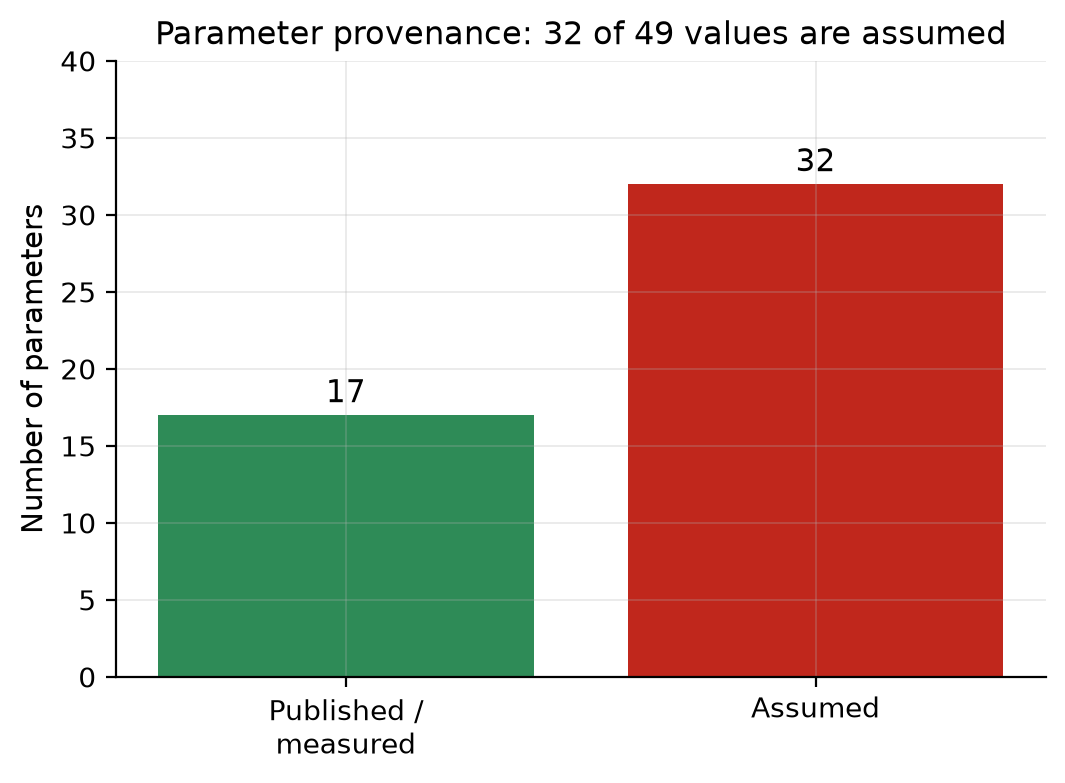
\includegraphics[width=0.98\columnwidth]{12_parameter_provenance.png}
    \caption{Provenance of the parameter set. Thirty-two of forty-nine values
    are engineering estimates, because the manufacturer publishes no motor map,
    gear ratio or usable battery capacity.}
    \label{fig:provenance}
\end{figure}

\section{Longitudinal Vehicle Model}
\label{sec:model}

\subsection{Force Balance}

The force the vehicle must deliver at the wheels to follow a demanded speed $v$
and acceleration $a$ is
\begin{equation}
F_{\mathrm{trac}} = F_{\mathrm{inertia}} + F_{\mathrm{run}}(v) + F_{\mathrm{grade}},
\label{eq:balance}
\end{equation}
where the inertia term accounts for the rotating masses of wheels, shafts and
rotor through a factor $\lambda$,
\begin{equation}
F_{\mathrm{inertia}} = \lambda\, m\, a ,
\qquad
F_{\mathrm{grade}} = m\, g \sin\alpha .
\end{equation}

\subsection{Running Resistance: Two Formulations}

Two formulations of the running resistance $F_{\mathrm{run}}$ are implemented,
and the difference between them is a result in its own right.

\subsubsection{Textbook Decomposition}

The decomposition taught in the standard
texts~\cite{ehsani2018,mitschke2014} separates the two physical mechanisms,
\begin{equation}
F_{\mathrm{run}}^{\mathrm{phys}}(v) =
\underbrace{f_r(v)\, m\, g \cos\alpha}_{\text{rolling}}
+ \underbrace{\tfrac{1}{2}\rho\, C_d A\, v^2}_{\text{aerodynamic}} ,
\label{eq:physical}
\end{equation}
with a speed-dependent rolling coefficient
$f_r(v) = f_{r0} + k v^2$. This form is what the report derives, and it is what
the traction diagram of Section~\ref{sec:characteristics} plots, because it
shows which mechanism dominates where.

\subsubsection{Regulatory Coastdown Form}

It is not, however, what the model uses to predict energy. Type approval does
not measure rolling resistance and aerodynamic drag separately. It rolls the
vehicle down from speed on a level test track and fits a
quadratic~\cite{gtr15,epacoastdown},
\begin{equation}
F_{\mathrm{run}}^{\mathrm{cd}}(v) = F_0 \frac{m}{m_{\mathrm{cd}}} + F_1 v + F_2 v^2 .
\label{eq:coastdown}
\end{equation}

This coastdown form is the default in the model because it is physically the
more complete description, for two reasons.

First, the linear term $F_1$ captures bearing, seal and driveline drag, for
which Equation~\ref{eq:physical} has no counterpart at all. An electric drive
unit cannot be disconnected during a coastdown, so its spin losses are
necessarily inside the measured coefficients.

Second, the quadratic term captures the aerodynamic drag the vehicle actually
experiences on the road, including wheel rotation and cooling airflow, both of
which a wind-tunnel drag coefficient excludes by construction.

The constant term $F_0$ is tyre rolling resistance, which is proportional to
normal load, so it is scaled by the ratio of the actual mass $m$ to the mass
$m_{\mathrm{cd}}$ at which the coastdown was performed. Without that correction
the model reports payload as very nearly free, because the kinetic energy that
extra mass adds is largely returned by regenerative braking.

\subsubsection{Comparison}

Table~\ref{tab:roadload} compares the two. The published drag coefficient of
$C_d = 0.219$ implies a drag area $C_d A = \SI{0.486}{\metre\squared}$, whereas
the coastdown quadratic implies $\SI{0.629}{\metre\squared}$, higher by
\SI{29}{\percent}. Both numbers are correct; they measure different things.
Using Equation~\ref{eq:physical} alone under-predicts the running resistance by
15 to \SI{19}{\percent} above \SI{80}{\kilo\metre\per\hour}, and the energy
demand by a comparable margin.

\begin{table}[H]
\centering
\caption{Running resistance from the two formulations. The textbook
decomposition has no linear term and uses a wind-tunnel drag coefficient, so it
falls progressively short as speed rises.}
\label{tab:roadload}
\footnotesize
\begin{tabular}{@{}rrrr@{}}
\toprule
\textbf{Speed} & \textbf{Coastdown} & \textbf{Textbook} & \textbf{Difference} \\
km/h & N & N & \% \\
\midrule
 30 & 157.7 & 168.2 & $+6.6$ \\
 50 & 214.9 & 207.0 & $-3.7$ \\
 80 & 344.5 & 301.7 & $-12.4$ \\
100 & 460.1 & 389.1 & $-15.4$ \\
130 & 677.3 & 556.6 & $-17.8$ \\
150 & 851.3 & 692.5 & $-18.6$ \\
\bottomrule
\end{tabular}
\end{table}

\subsection{Powertrain}

\subsubsection{Torque and Power Envelope}

A traction machine is operated in two regions. Below the corner point the
current limit binds and the torque is constant; above it the voltage limit
binds and the machine enters field weakening at constant
power~\cite{sarlioglu2017},
\begin{equation}
T_{\max}(\omega) =
\begin{cases}
T_{\mathrm{pk}}, & \omega \le \omega_b, \\[4pt]
\dfrac{P_{\mathrm{pk}}}{\omega}, & \omega_b < \omega \le \omega_{\max},
\end{cases}
\label{eq:envelope}
\end{equation}
with the corner point at $\omega_b = P_{\mathrm{pk}} / T_{\mathrm{pk}}$. For
this vehicle $\omega_b$ corresponds to \SI{4729}{rpm}, which is
\SI{65.8}{\kilo\metre\per\hour} at the wheels. The tractive force available at
the road is
\begin{equation}
F_{\mathrm{mot}}(v) = \frac{T_{\max}(\omega)\, i_g\, \eta_g}{r_w},
\qquad
\omega = \frac{v\, i_g}{r_w} .
\end{equation}

\subsubsection{Loss Model}

A single fixed efficiency is not adequate here. A legislative cycle spends most
of its time at light load, where a real drive unit is markedly less efficient
than at its rated point, so a constant value would misstate the cycle energy in
whichever direction it was calibrated. The combined motor-and-inverter loss is
therefore represented by the four-term model of Larminie and
Lowry~\cite{larminie2012},
\begin{equation}
P_{\mathrm{loss}} = k_c T^2 + k_i \omega + k_w \omega^3 + P_0 ,
\label{eq:loss}
\end{equation}
whose terms are respectively copper (current-dependent), iron
(flux-dependent), windage, and constant electronics loss.

The four coefficients were fitted by least squares to seven operating points
typical of a liquid-cooled automotive permanent-magnet machine: approximately
\SI{97}{\percent} peak efficiency, \SI{92.5}{\percent} at peak power,
\SI{88}{\percent} at light load and high speed corresponding to motorway
cruise, and \SI{80}{\percent} at light load and low speed. The resulting map is
shown in Figure~\ref{fig:efficiency}. All four coefficients are \asm{assumed}.

\subsection{Battery}

The pack is modelled as a state-of-charge dependent open-circuit voltage in
series with a constant internal resistance, the \emph{Rint} equivalent
circuit~\cite{he2011,plett2004},
\begin{equation}
P_{\mathrm{term}} = V_{oc}(z)\, I - I^2 R_i ,
\end{equation}
which is solved for the current drawn at a demanded terminal power,
\begin{equation}
I = \frac{V_{oc} - \sqrt{V_{oc}^2 - 4 R_i P_{\mathrm{term}}}}{2 R_i} .
\label{eq:current}
\end{equation}
The radicand turns negative beyond the resistance-limited power ceiling
$V_{oc}^2 / 4R_i$, which the implementation reports as a limit rather than
silently returning a complex value.

State of charge is tracked in ampere-hours rather than in energy. This matters:
it charges the ohmic loss against the pack instead of ignoring it, and counts
it correctly twice on a cycle with heavy regeneration, once on the way out and
once on the way back in. The pack capacity is sized so that
$\int V_{oc}\,\mathrm{d}q$ across the usable window equals the nameplate usable
energy, giving \SI{175.3}{\ampere\hour} at a window-averaged open-circuit
voltage of \SI{342.3}{\volt}. A slow discharge then returns
\SI{59.96}{\kilo\watt\hour} at the terminals against a \SI{60.0}{\kilo\watt\hour}
nameplate, the difference being the ohmic loss.

The LFP open-circuit voltage curve is \asm{assumed}, scaled from published cell
data. It rises only about \SI{6}{\percent} between \SI{25}{\percent} and
\SI{85}{\percent} state of charge, which is the characteristic flat plateau of
the chemistry.

\subsection{Simulation Method}

The simulation is quasi-static and backward-facing, the standard approach for
energy and range work~\cite{guzzella2013}: the speed trace is the input, and
the model asks what the powertrain must do to follow it. No driver model is
required. Within each one-second step the forces are evaluated at the mid-point
speed
\begin{equation}
\bar v = \tfrac{1}{2}\left(v_k + v_{k+1}\right),
\qquad
a_k = \frac{v_{k+1} - v_k}{\Delta t},
\end{equation}
which makes the integration second-order rather than first-order accurate.

Every limit, mechanical and electrical, is resolved \emph{before} the step is
committed. If the motor envelope, the tyre adhesion limit, the battery power
rating or the remaining charge cannot deliver what the trace demands, the model
substitutes the acceleration that is actually achievable and flags the step. It
never reports a vehicle following a trace on energy the battery did not supply.
Over the WLTC the vehicle meets the demand at every one of the 1800 steps, with
a peak tracking error of \SI{0}{\kilo\metre\per\hour}.

\section{Speed and Acceleration Characteristics}
\label{sec:characteristics}

\subsection{Tyre Adhesion Limit}

The force available at the road is the lesser of what the machine can produce
and what the driven tyres can transmit. For a rear-wheel-drive vehicle the
second of these binds first, and the problem is implicit: accelerating
transfers load onto the driven axle, which raises the adhesion limit, which
permits more acceleration. The normal load on the rear axle is
\begin{equation}
N_r = \chi\, m\, g \cos\alpha + \frac{m\, a\, h}{L} ,
\end{equation}
the adhesion limit is $F_{\mathrm{adh}} = \mu N_r$, and the acceleration is
$a = (F - F_{\mathrm{res}})/(\lambda m)$. Eliminating $a$ gives a closed form,
which the implementation solves directly rather than iterating:
\begin{equation}
F_{\mathrm{adh}} =
\frac{\mu \chi m g \cos\alpha - \dfrac{\mu h F_{\mathrm{res}}}{L \lambda}}
     {1 - \dfrac{\mu h}{L \lambda}} .
\label{eq:adhesion}
\end{equation}

This is not a refinement of secondary importance. At rest the tyres can
transmit \SI{9.30}{\kilo\newton} while the motor could deliver
\SI{11.15}{\kilo\newton}, so the vehicle is traction-limited for roughly the
first third of its run to \SI{100}{\kilo\metre\per\hour}. A model that omits
the load transfer predicts an acceleration time about \SI{15}{\percent}
optimistic.

\subsection{Traction Diagram}

Figure~\ref{fig:traction} plots the available force against the running
resistance. The motor envelope is flat to the corner point at
\SI{65.8}{\kilo\metre\per\hour} and falls as $1/v$ thereafter. The adhesion
limit, drawn in the assumption colour because it depends on an estimated
friction coefficient, cuts below the envelope up to about
\SI{78}{\kilo\metre\per\hour}. The dashed curve is the textbook decomposition
of Equation~\ref{eq:physical}, shown for comparison; the gap between it and the
solid total resistance is the shortfall quantified in
Table~\ref{tab:roadload}.

\begin{figure}[H]
    \centering
    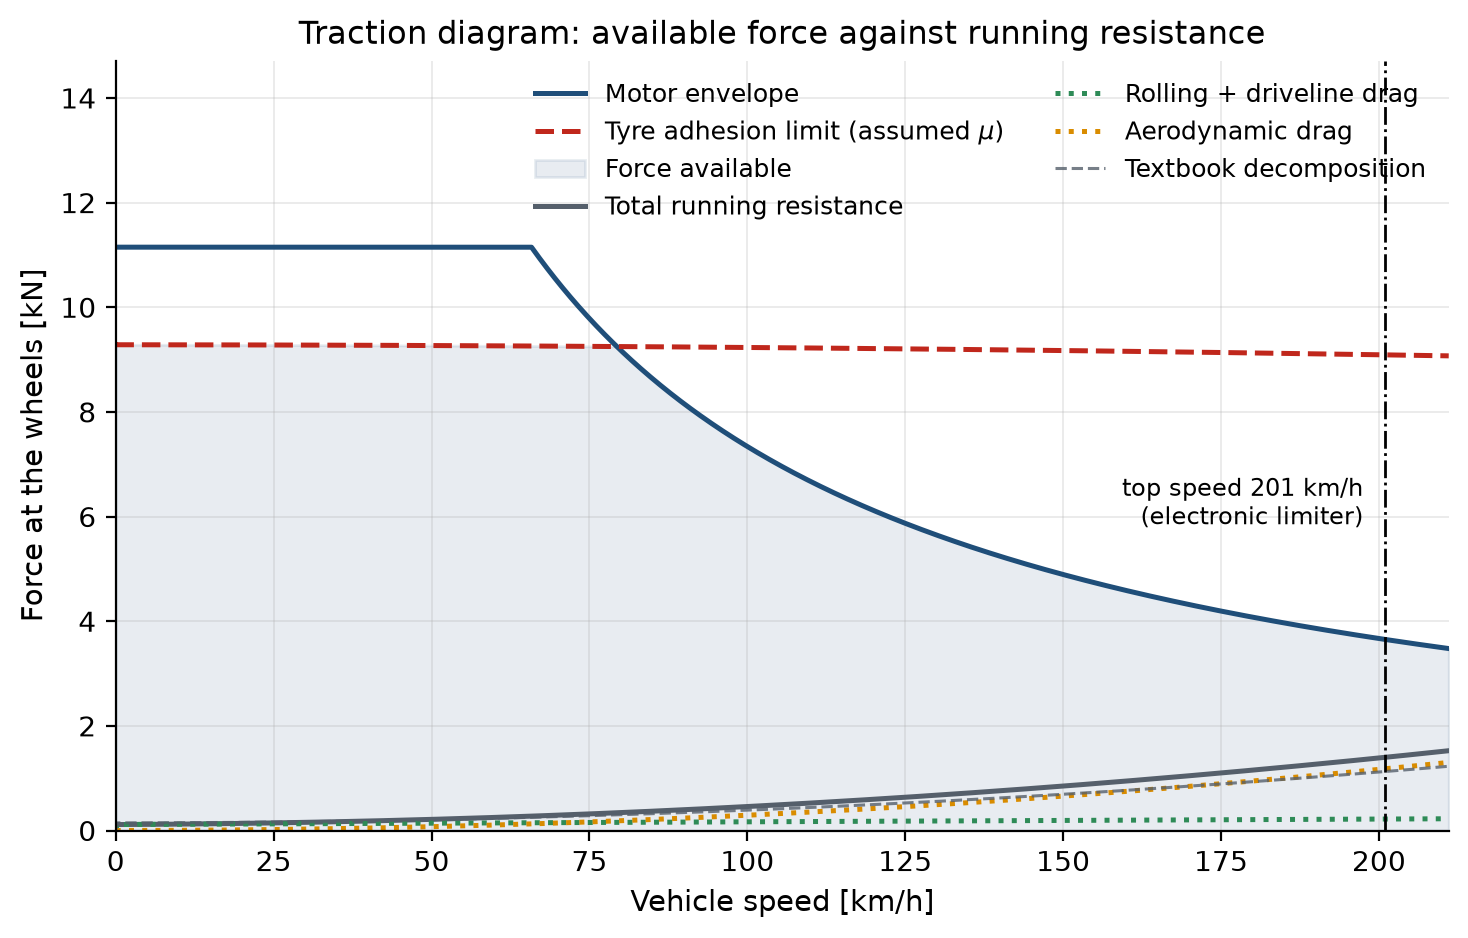
\includegraphics[width=\columnwidth]{01_traction_diagram.png}
    \caption{Traction diagram. Available force against running resistance, with
    the tyre adhesion limit and the textbook road-load decomposition shown for
    comparison.}
    \label{fig:traction}
\end{figure}

\subsection{Acceleration Characteristic}

The maximum acceleration at each speed follows directly,
\begin{equation}
a_{\max}(v) = \frac{\min\!\left[F_{\mathrm{mot}}(v),\, F_{\mathrm{adh}}(v)\right]
 - F_{\mathrm{run}}(v)}{\lambda m} .
\label{eq:amax}
\end{equation}
The full-throttle launch is obtained by integrating
\begin{equation}
t = \int_{0}^{v} \frac{\mathrm{d}u}{a_{\max}(u)} ,
\label{eq:launch}
\end{equation}
on a fine speed grid, which is numerically far better behaved near standstill
than stepping in time. Figure~\ref{fig:accel} shows both, with the
tyre-limited region shaded on the left panel and the benchmark times marked on
the right. Table~\ref{tab:perf} collects the results.

\begin{figure}[H]
    \centering
    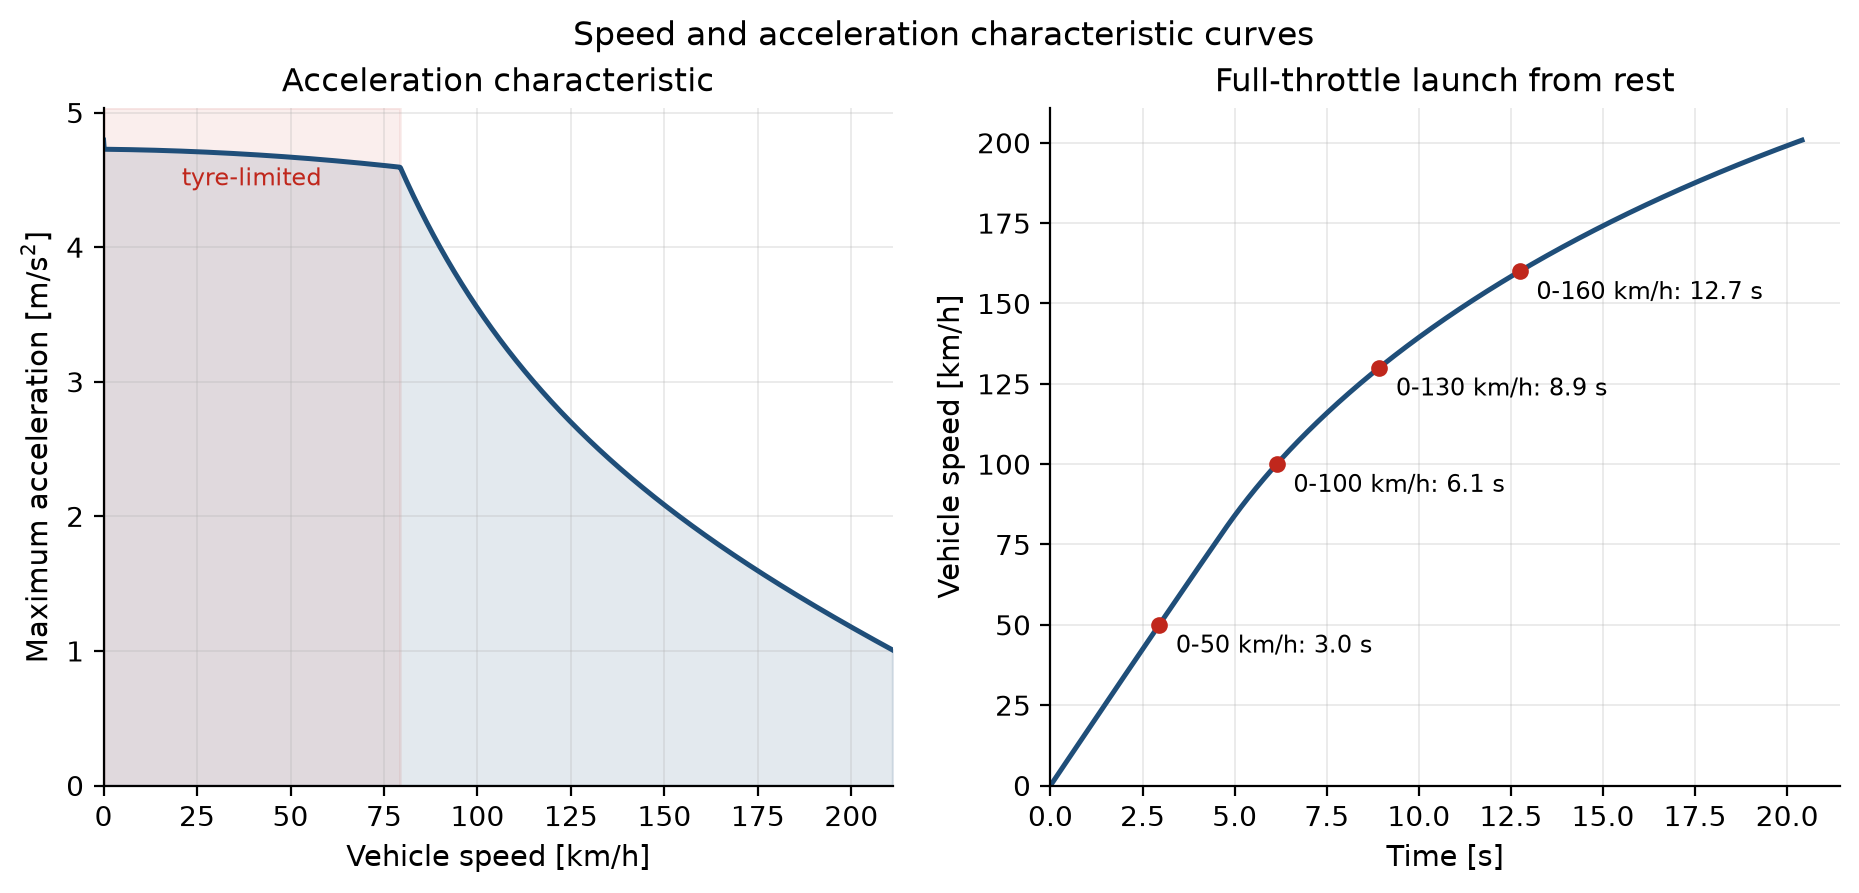
\includegraphics[width=\columnwidth]{02_acceleration_characteristic.png}
    \caption{Speed and acceleration characteristic curves. Left: maximum
    acceleration against speed, with the tyre-limited region shaded. Right:
    the full-throttle launch from rest.}
    \label{fig:accel}
\end{figure}

\begin{table}[H]
\centering
\caption{Predicted performance characteristics.}
\label{tab:perf}
\footnotesize
\begin{tabular}{@{}lrl@{}}
\toprule
\textbf{Quantity} & \textbf{Value} & \textbf{Unit} \\
\midrule
Maximum acceleration from rest & 4.79  & m/s$^2$ \\
Maximum tractive force         & 9.30  & kN \\
Maximum wheel power            & 203.8 & kW \\
0--50 km/h                     & 2.95  & s \\
0--100 km/h                    & 6.14  & s \\
0--130 km/h                    & 8.93  & s \\
0--160 km/h                    & 12.74 & s \\
Top speed                      & 201   & km/h \\
\bottomrule
\end{tabular}
\end{table}

\subsection{Top Speed and Gradeability}

Three distinct constraints can cap the top speed of a battery-electric vehicle,
and which one binds is a design statement worth reporting rather than a number
to be quoted in isolation. They are the tractive force balance, the maximum
mechanical speed of the machine, and the electronic limiter.

For this vehicle the limiter binds, at \SI{201}{\kilo\metre\per\hour}. Removing
it, the machine reaches its \asm{\SI{17900}{rpm}} ceiling at
\SI{249}{\kilo\metre\per\hour} with tractive force still in reserve, so the
force balance never binds at all. The implementation reports which of the three
is active.

Gradeability follows from setting the acceleration to zero and solving the
force balance for the slope. Figure~\ref{fig:power} shows the power envelope
and the maximum climbable gradient against speed. The vehicle will pull away on
a gradient well beyond anything found on a public road, which is characteristic
of electric traction and its full torque from rest.

\begin{figure}[H]
    \centering
    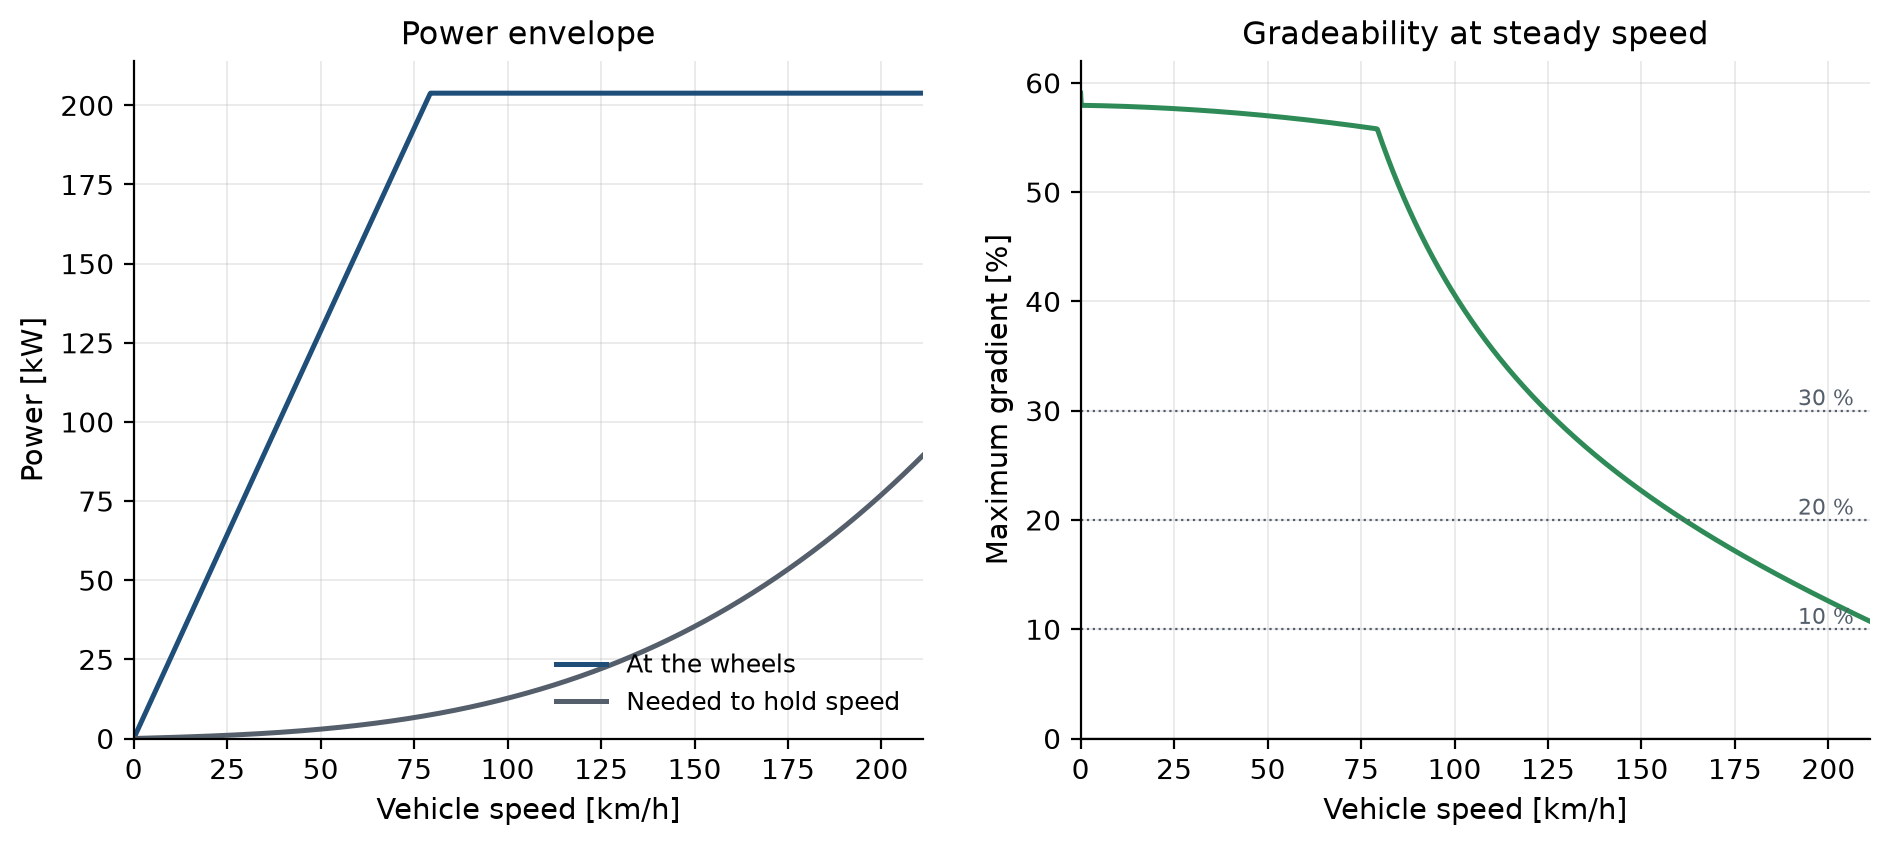
\includegraphics[width=\columnwidth]{03_power_and_gradeability.png}
    \caption{Power envelope at the wheels and maximum climbable gradient at
    steady speed.}
    \label{fig:power}
\end{figure}

\begin{figure}[H]
    \centering
    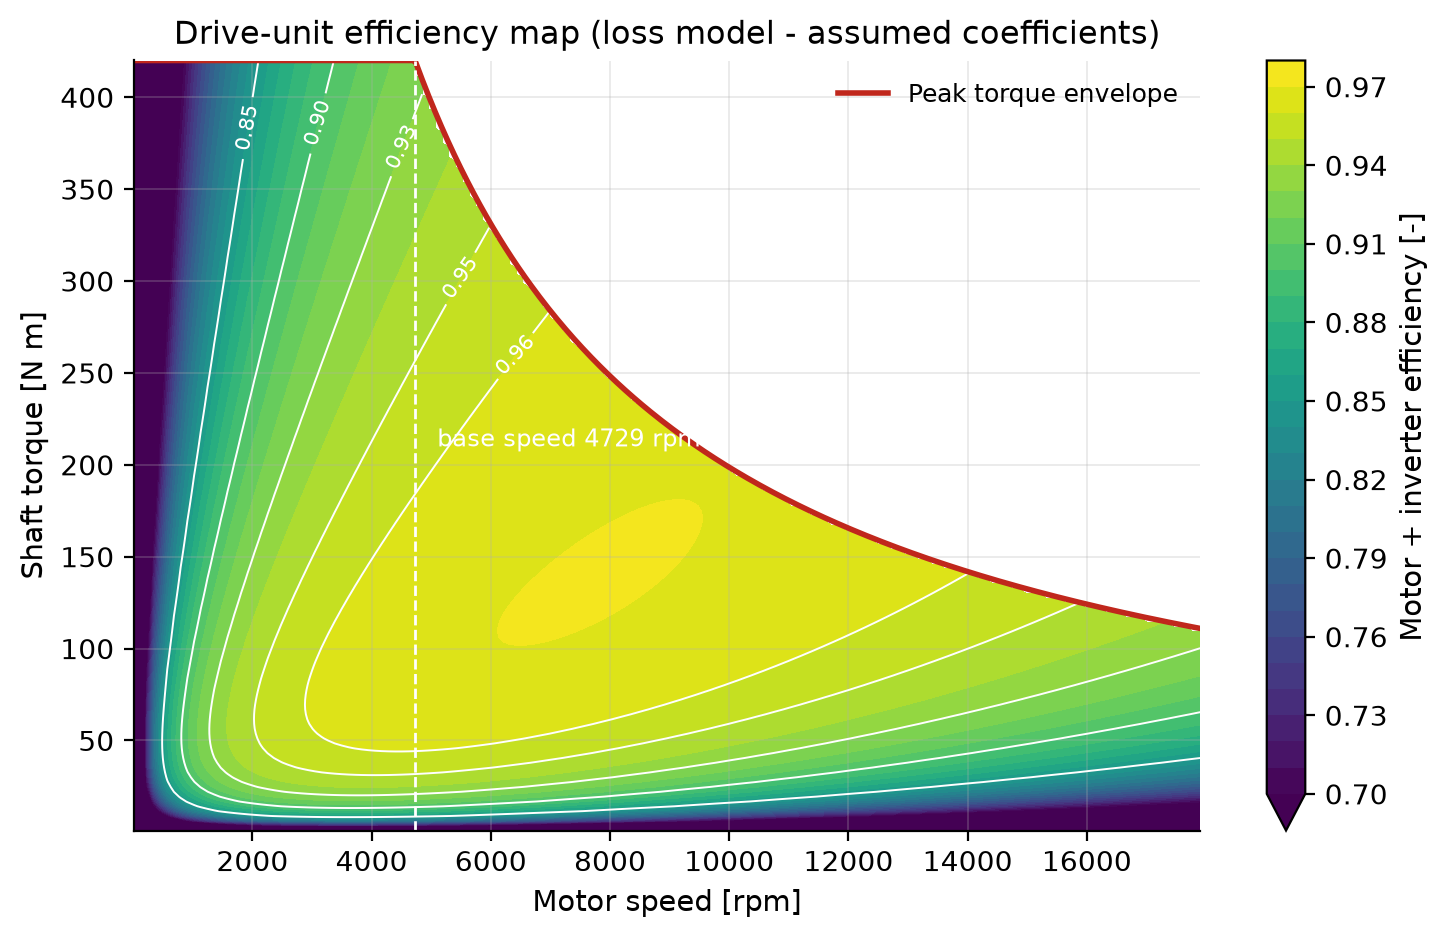
\includegraphics[width=\columnwidth]{04_efficiency_map.png}
    \caption{Combined motor and inverter efficiency map from
    Equation~\ref{eq:loss}, with the peak torque envelope overlaid. The
    coefficients are \asm{assumed}, fitted to seven representative operating
    points.}
    \label{fig:efficiency}
\end{figure}

\section{Driving Profile}
\label{sec:cycle}

\subsection{Choice of Cycle}

The WLTC Class~3b cycle was selected because the vehicle's own published range
is certified on it~\cite{gtr15}, so the model and its reference describe the
same drive. Comparing a prediction made on one profile against a figure
certified on another would confound the model error with the difference between
the cycles.

The cycle runs for \SI{1800}{\second} over \SI{23.27}{\kilo\metre} in four
phases of rising speed, labelled Low, Medium, High and Extra-high, reaching a
maximum of \SI{131.3}{\kilo\metre\per\hour}. Figure~\ref{fig:cycle} shows the
speed and acceleration traces with the phases marked.

\subsection{Profile Synthesis}

The official second-by-second table of the WLTC is not reproduced here.
Instead the profile is \asm{synthesised} from the published phase statistics.
For each phase the construction specifies a sequence of speed levels, ramps
linearly between them at realistic rates, and solves for the hold durations.
Two linear constraints on the $n$ non-zero hold durations $t$ fix the phase
duration and its distance,
\begin{equation}
\sum_i t_i = T_{\mathrm{drive}} - T_{\mathrm{ramp}},
\quad
\sum_i v_i t_i = D - D_{\mathrm{ramp}} ,
\label{eq:holds}
\end{equation}
which for $n > 2$ is underdetermined. The solution closest to a nominal
distribution is taken by solving the equality-constrained least-squares problem
$\min \lVert t - t_0 \rVert^2$ subject to $At = b$ through its Lagrangian,
$t = t_0 + A^{\mathsf T}(AA^{\mathsf T})^{-1}(b - At_0)$.

The resulting trace is not the official one second by second, but every
published statistic is reproduced to within half a per cent, as
Table~\ref{tab:cycle} shows. More importantly, the energy result does not
depend on the shape of the synthetic trace: sweeping the acceleration rates
across their whole plausible span moves the predicted consumption by only
\SI{1.9}{\percent}. Supplying the official table overrides the synthesis
automatically.

\begin{table}[H]
\centering
\caption{Synthesised WLTC Class~3b against the published statistics.}
\label{tab:cycle}
\footnotesize
\begin{tabular}{@{}lrrr@{}}
\toprule
\textbf{Statistic} & \textbf{Generated} & \textbf{Published} & \textbf{Dev.} \\
\midrule
Duration (s)            & 1800.0  & 1800.0  & $+0.00$\,\% \\
Distance (km)           & 23.268  & 23.266  & $+0.01$\,\% \\
Maximum speed (km/h)    & 131.30  & 131.30  & $+0.00$\,\% \\
Mean speed (km/h)       & 46.54   & 46.50   & $+0.08$\,\% \\
Stop time (s)           & 243.0   & 242.0   & $+0.41$\,\% \\
\midrule
Low phase (km)          & 3.096   & 3.095   & $+0.02$\,\% \\
Medium phase (km)       & 4.756   & 4.756   & $+0.00$\,\% \\
High phase (km)         & 7.162   & 7.162   & $-0.00$\,\% \\
Extra-high phase (km)   & 8.254   & 8.254   & $-0.00$\,\% \\
\bottomrule
\end{tabular}
\end{table}

\begin{figure}[H]
    \centering
    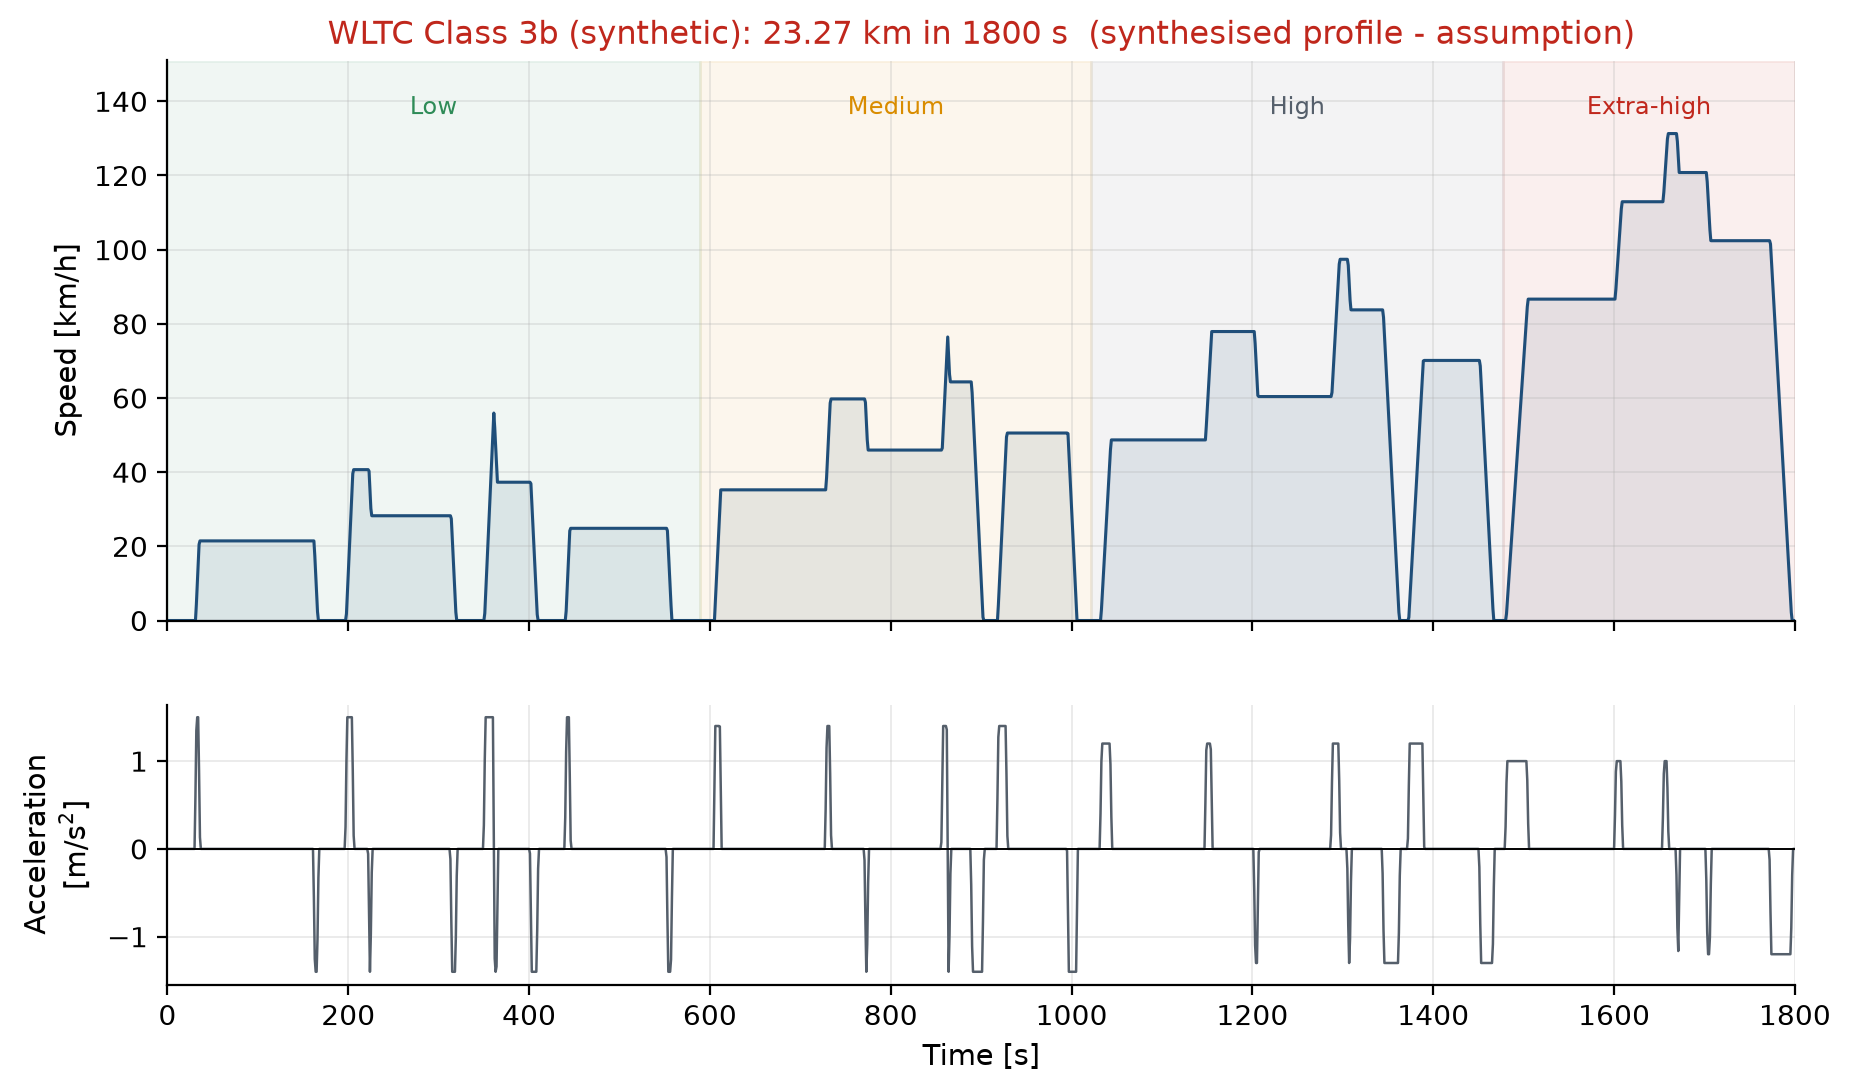
\includegraphics[width=\columnwidth]{05_driving_cycle.png}
    \caption{WLTC Class~3b speed and acceleration traces, with the four phases
    shaded.}
    \label{fig:cycle}
\end{figure}

\subsection{Comparison Cycle}

The New European Driving Cycle (NEDC) is also implemented, reconstructed
directly from its regulatory segment table~\cite{unece83}. Because that table
specifies the cycle as idle, constant-acceleration and constant-speed segments,
the reconstruction is deterministic. It yields \SI{1180}{\second} and
\SI{10.975}{\kilo\metre} against the official \SI{11.007}{\kilo\metre}, low by
\SI{0.29}{\percent}; the residual lies in the published urban segment table,
whose durations sum to \SI{194}{\second} rather than \SI{195}{\second}.

The NEDC serves to show how much the choice of profile alone changes the
answer, and is discussed in Section~\ref{sec:validation}. Its much gentler
speed and acceleration content, visible in Figure~\ref{fig:nedc}, is the reason
it was replaced by the WLTP~\cite{pavlovic2016,tsiakmakis2019}. Where the WLTC
is built from irregular micro-trips with continuously varying speed, the NEDC
consists of repeated trapezoidal segments at constant acceleration, a profile
no driver produces and one that understates both the transient losses and the
high-speed drag a vehicle actually meets.

\begin{figure}[H]
    \centering
    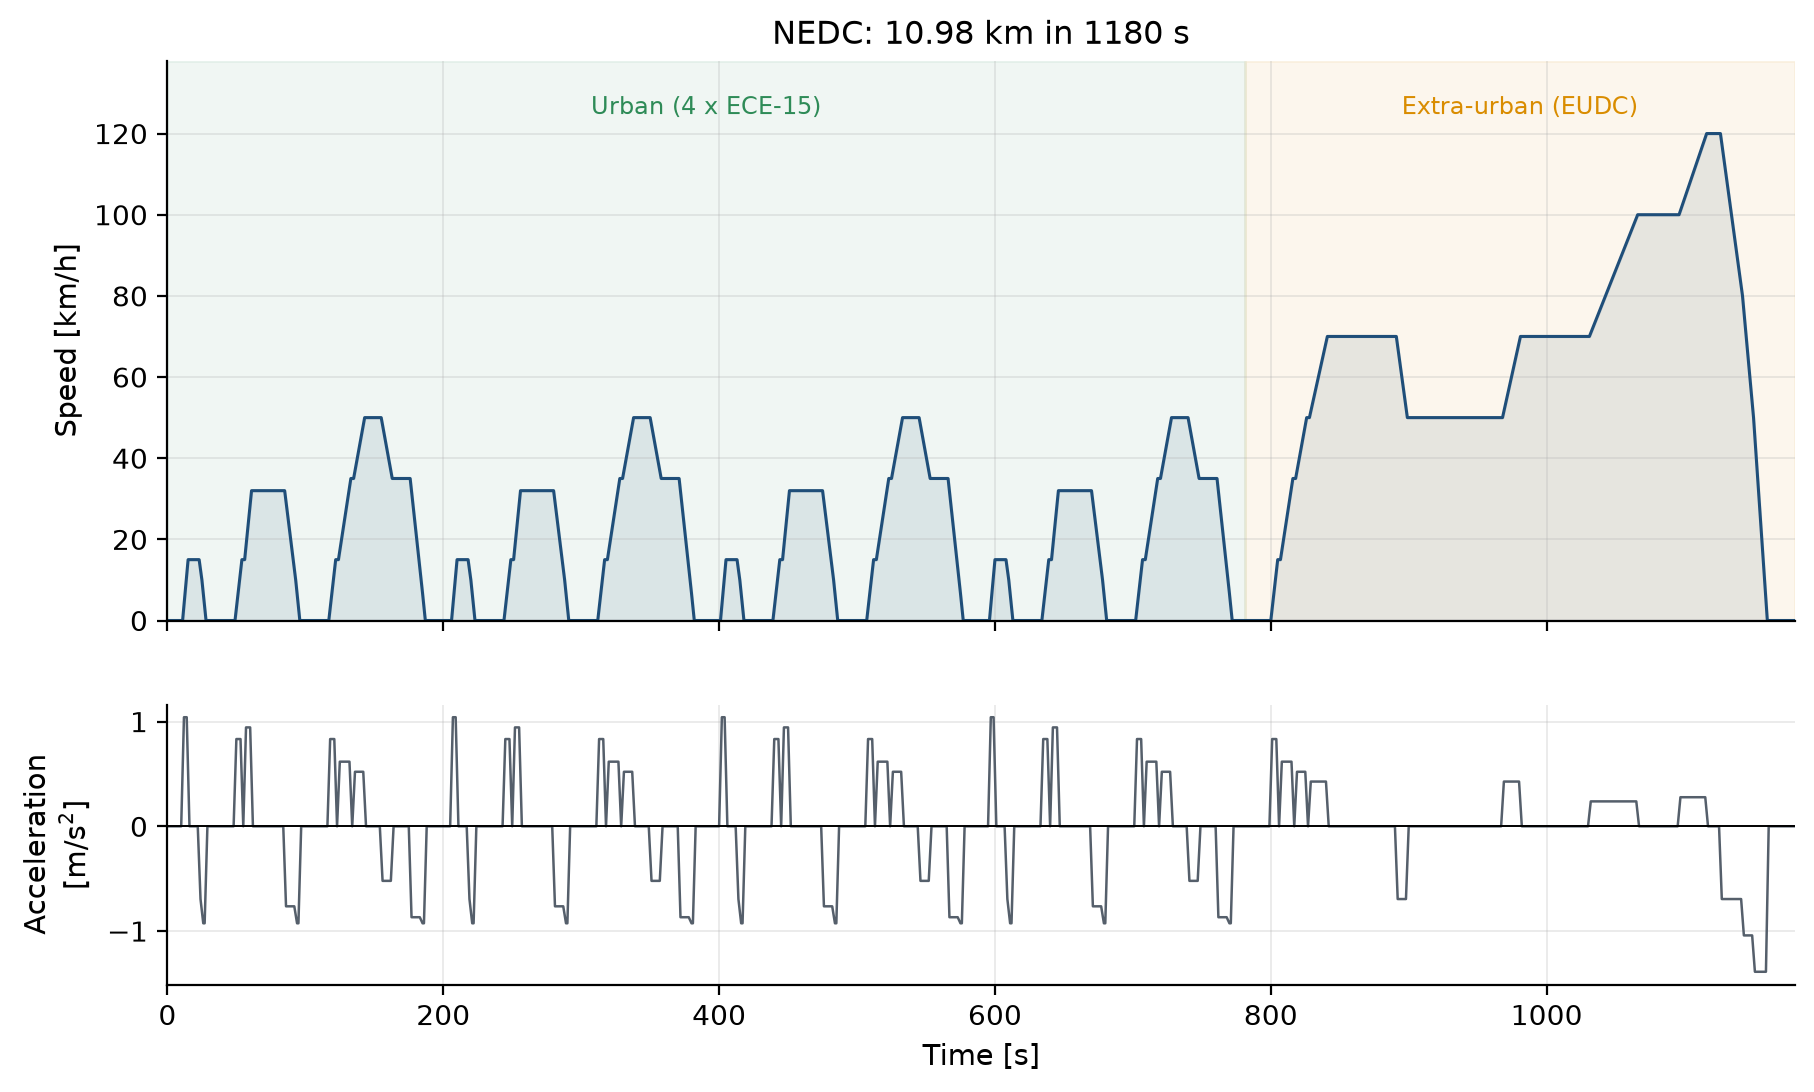
\includegraphics[width=\columnwidth]{13_nedc_cycle.png}
    \caption{NEDC speed and acceleration traces, reconstructed from the
    regulatory segment table. The four repeated urban segments are followed by
    a single extra-urban phase.}
    \label{fig:nedc}
\end{figure}

\section{Cycle Simulation and Energy Balance}
\label{sec:simulation}

\subsection{Results Over One Cycle}

Over one pass of the WLTC the vehicle covers \SI{23.27}{\kilo\metre} and draws
\SI{2.665}{\kilo\watt\hour} net from the battery, giving a consumption of
\SI{11.45}{\kWhph} at the terminals.
Regenerative braking returns \SI{24.6}{\percent} of the traction energy.
Figure~\ref{fig:simulation} shows the speed, battery power and state of charge
over the cycle. The demanded trace is entirely hidden behind the achieved one,
which is the point: the powertrain follows the profile at every step.

\begin{figure}[H]
    \centering
    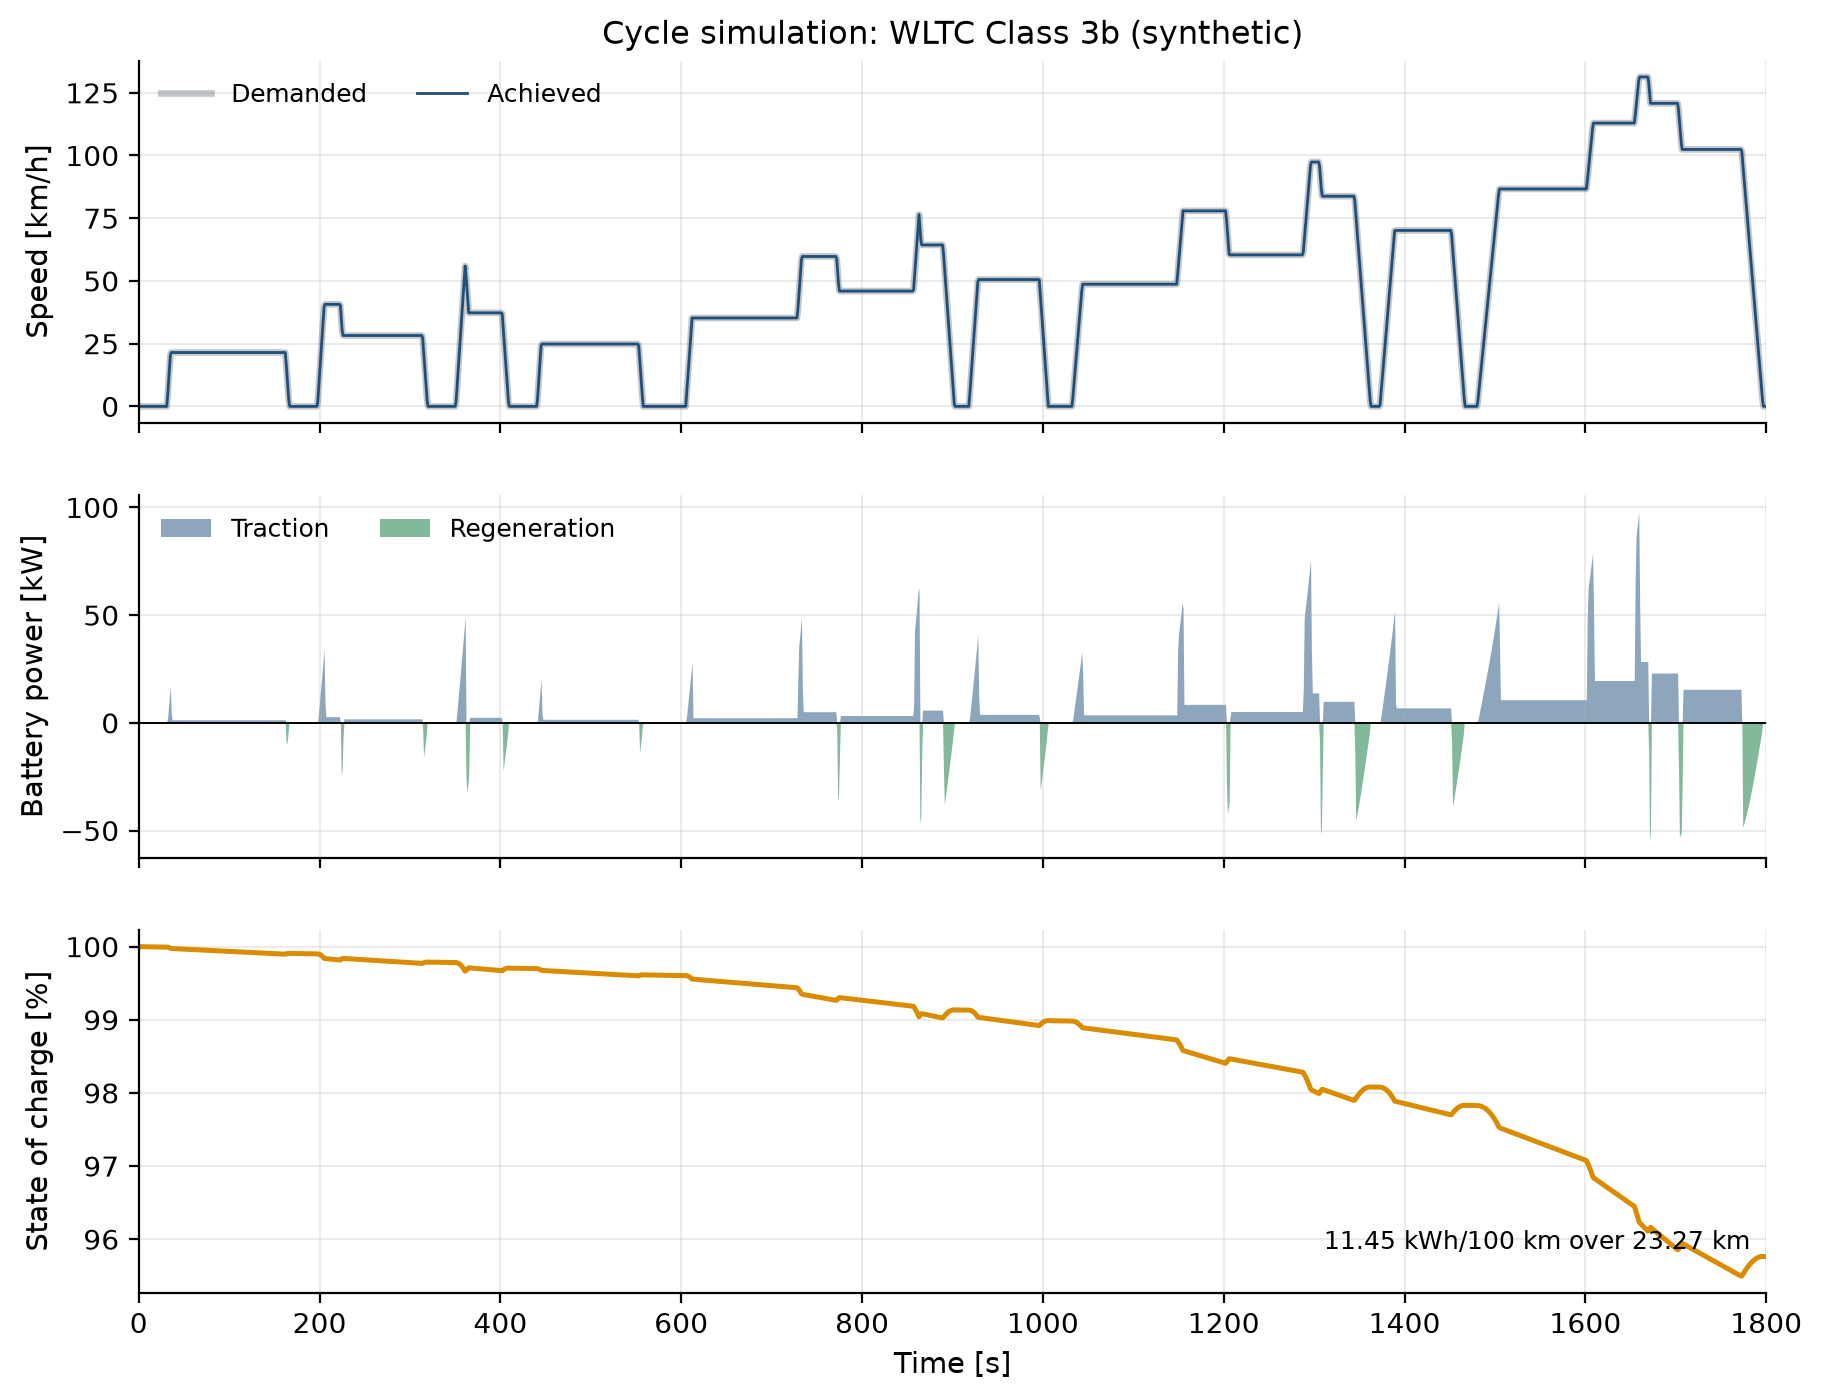
\includegraphics[width=\columnwidth]{06_cycle_simulation.png}
    \caption{Cycle simulation. Demanded and achieved speed, battery power split
    into traction and regeneration, and state of charge.}
    \label{fig:simulation}
\end{figure}

\subsection{Energy Demand by Phase}

Because the four WLTC phases differ so widely in speed, the cycle can be read
as four separate drives. Table~\ref{tab:phases} reports the consumption of
each.

The specific consumption rises from \SI{81.5}{\Whpkm} in the
Low phase to \SI{156.0}{\Whpkm} in the Extra-high phase,
very nearly a doubling. Two mechanisms drive this. Aerodynamic drag grows with
the square of speed and dissipates energy that cannot be recovered, and the
share of traction energy returned by regeneration falls from
\SI{27.7}{\percent} to \SI{17.0}{\percent} because a high-speed phase spends
proportionally less of its time braking.

The consequence for a driver is direct: the Extra-high phase contributes
\SI{35}{\percent} of the cycle distance but \SI{48}{\percent} of its energy.
A journey conducted entirely at motorway speed will fall well short of the
certified range even before any auxiliary load is considered, and
Figure~\ref{fig:cruise} quantifies that case.

\begin{table}[H]
\centering
\caption{Energy demand by WLTC phase. Specific consumption nearly doubles
between the Low and Extra-high phases.}
\label{tab:phases}
\footnotesize
\begin{tabular}{@{}lrrrrr@{}}
\toprule
\textbf{Phase} & \textbf{Dist.} & \textbf{$v_{\mathrm{avg}}$} & \textbf{Energy}
 & \textbf{Spec.} & \textbf{Regen} \\
 & km & km/h & kWh & Wh/km & \% \\
\midrule
Low        & 3.096 & 18.9 & 0.2524 &  81.5 & 27.7 \\
Medium     & 4.756 & 39.5 & 0.3959 &  83.2 & 30.0 \\
High       & 7.162 & 56.7 & 0.7286 & 101.7 & 27.9 \\
Extra-high & 8.254 & 92.0 & 1.2878 & 156.0 & 17.0 \\
\midrule
\textbf{Total} & \textbf{23.268} & \textbf{46.5} & \textbf{2.6646}
 & \textbf{114.5} & \textbf{24.6} \\
\bottomrule
\end{tabular}
\end{table}

\subsection{Energy Balance}

Table~\ref{tab:energy} decomposes where the energy goes. The four terms close
against the net battery energy to within \SI{1e-14}{\kilo\watt\hour}, which is
a check on the book-keeping rather than a coincidence: the drive-unit loss is
measured directly as the difference between electrical and wheel power in each
step, not inferred by subtracting the other terms.

The road load dominates at \SI{77}{\percent} of the total. Drive-unit losses
account for \SI{17}{\percent}, the auxiliary load for \SI{5.6}{\percent}, and
friction braking for only \SI{0.3}{\percent}, the last because the cycle's
decelerations are gentle enough that the motor absorbs nearly all of them
within its regeneration limit.

\begin{table}[H]
\centering
\caption{Energy balance over one WLTC cycle. The four expenditure terms close
exactly against the net battery energy.}
\label{tab:energy}
\footnotesize
\begin{tabular}{@{}lrr@{}}
\toprule
\textbf{Term} & \textbf{kWh} & \textbf{Share} \\
\midrule
Road load (rolling, driveline, drag) & 2.0608 & 77.3\,\% \\
Drive-unit losses                    & 0.4450 & 16.7\,\% \\
Auxiliaries                          & 0.1500 &  5.6\,\% \\
Friction brakes                      & 0.0088 &  0.3\,\% \\
\midrule
\textbf{Net from the battery}        & \textbf{2.6646} & 100\,\% \\
\bottomrule
\end{tabular}
\end{table}

\begin{figure}[H]
    \centering
    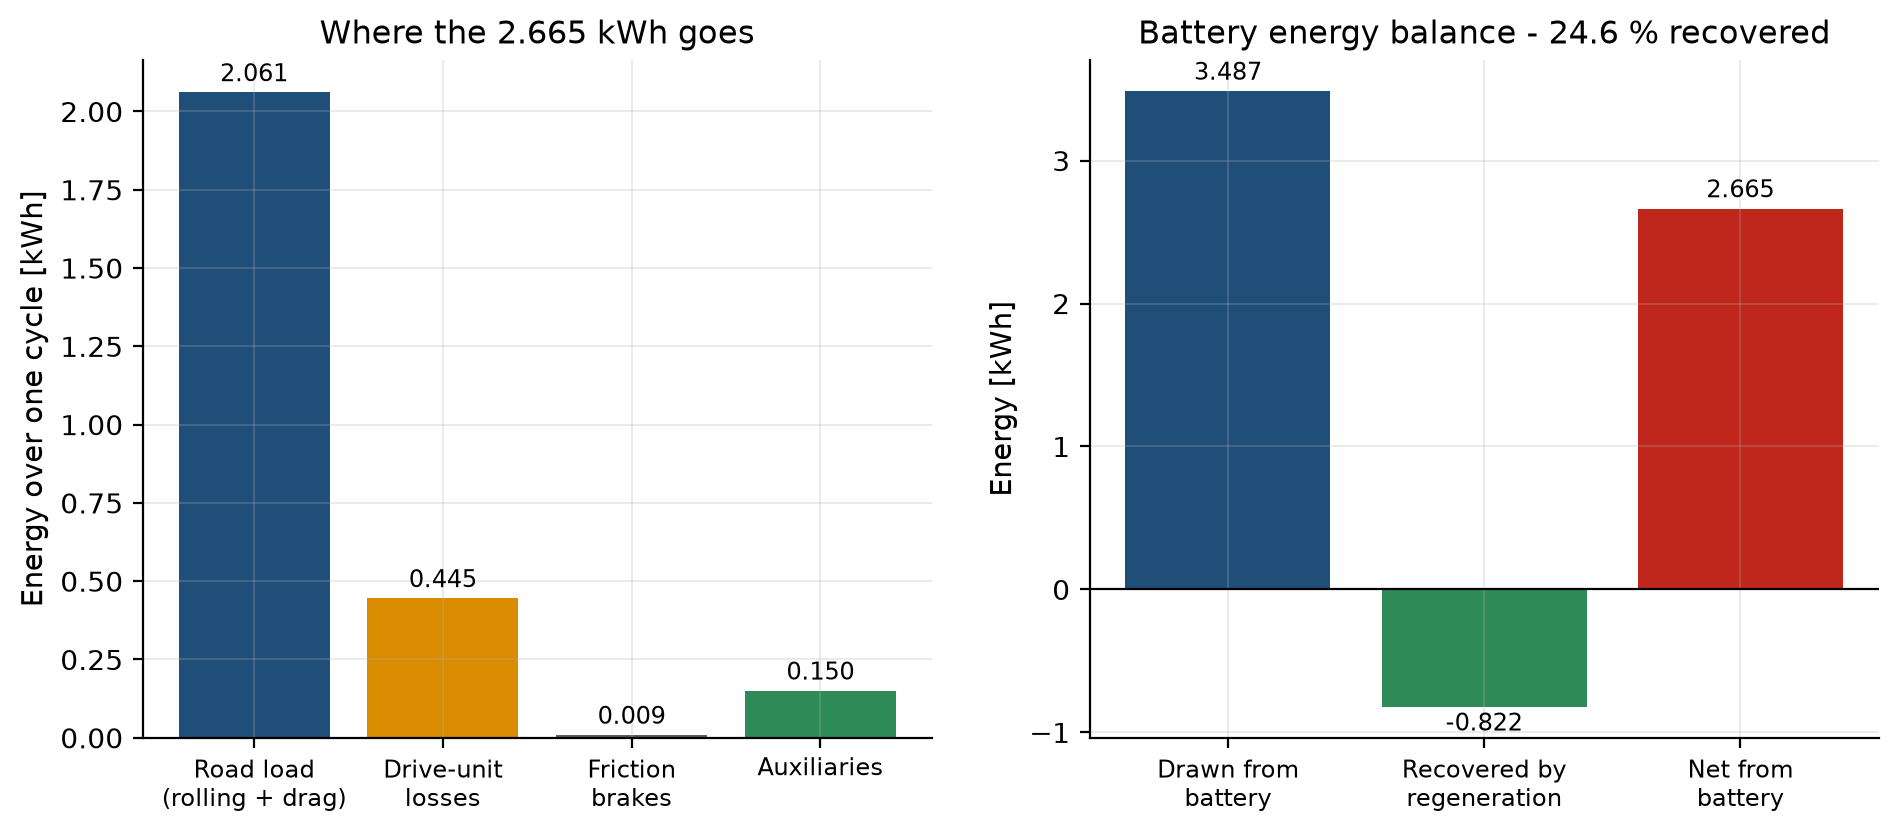
\includegraphics[width=\columnwidth]{07_energy_balance.png}
    \caption{Energy expenditure over one cycle and the battery energy balance,
    showing the share recovered by regeneration.}
    \label{fig:energy}
\end{figure}

\section{Range on a Full Battery}
\label{sec:range}

\subsection{Two Independent Methods}

Range is computed two ways, which serves as a cross-check on the energy
accounting.

The \emph{analytic} method divides the usable battery energy by the consumption
per kilometre. The \emph{integrated} method repeats the cycle, carrying the
state of charge forward, until the usable window is exhausted, so that it sees
the ohmic loss grow as the open-circuit voltage falls towards the end of the
discharge.

Both divisions must be performed at the open-circuit level, because that is
where the usable energy is defined: coulomb counting makes the state-of-charge
window hold $\int V_{oc}\,\mathrm{d}q$, not $\int P_{\mathrm{term}}\,\mathrm{d}t$.
Dividing the usable energy by the terminal consumption instead would overstate
the range by roughly the ohmic loss, and that unit error would then masquerade
as a disagreement between the two methods.

With both on the same footing they agree to \SI{0.64}{\percent}, the integrated
method giving the shorter range, which is the direction the physics demands.
Table~\ref{tab:range} gives the figures and Figure~\ref{fig:range} the
discharge trace.

\begin{table}[H]
\centering
\caption{Range on a full battery over the WLTC Class~3b cycle.}
\label{tab:range}
\footnotesize
\begin{tabular}{@{}lrl@{}}
\toprule
\textbf{Quantity} & \textbf{Value} & \textbf{Unit} \\
\midrule
Range, integrated method        & 508.3 & km \\
Range, analytic method          & 511.6 & km \\
Disagreement between methods    & $-0.64$ & \% \\
Consumption at the terminals    & 114.5 & Wh/km \\
Consumption at open circuit     & 117.4 & Wh/km \\
Usable battery energy           & 60.0  & kWh \\
Cycle repetitions to empty      & 21.8  & -- \\
\midrule
\textbf{Published WLTP range}   & \textbf{513.0} & \textbf{km} \\
\textbf{Deviation}              & $\mathbf{-0.92}$ & \textbf{\%} \\
\bottomrule
\end{tabular}
\end{table}

\begin{figure}[H]
    \centering
    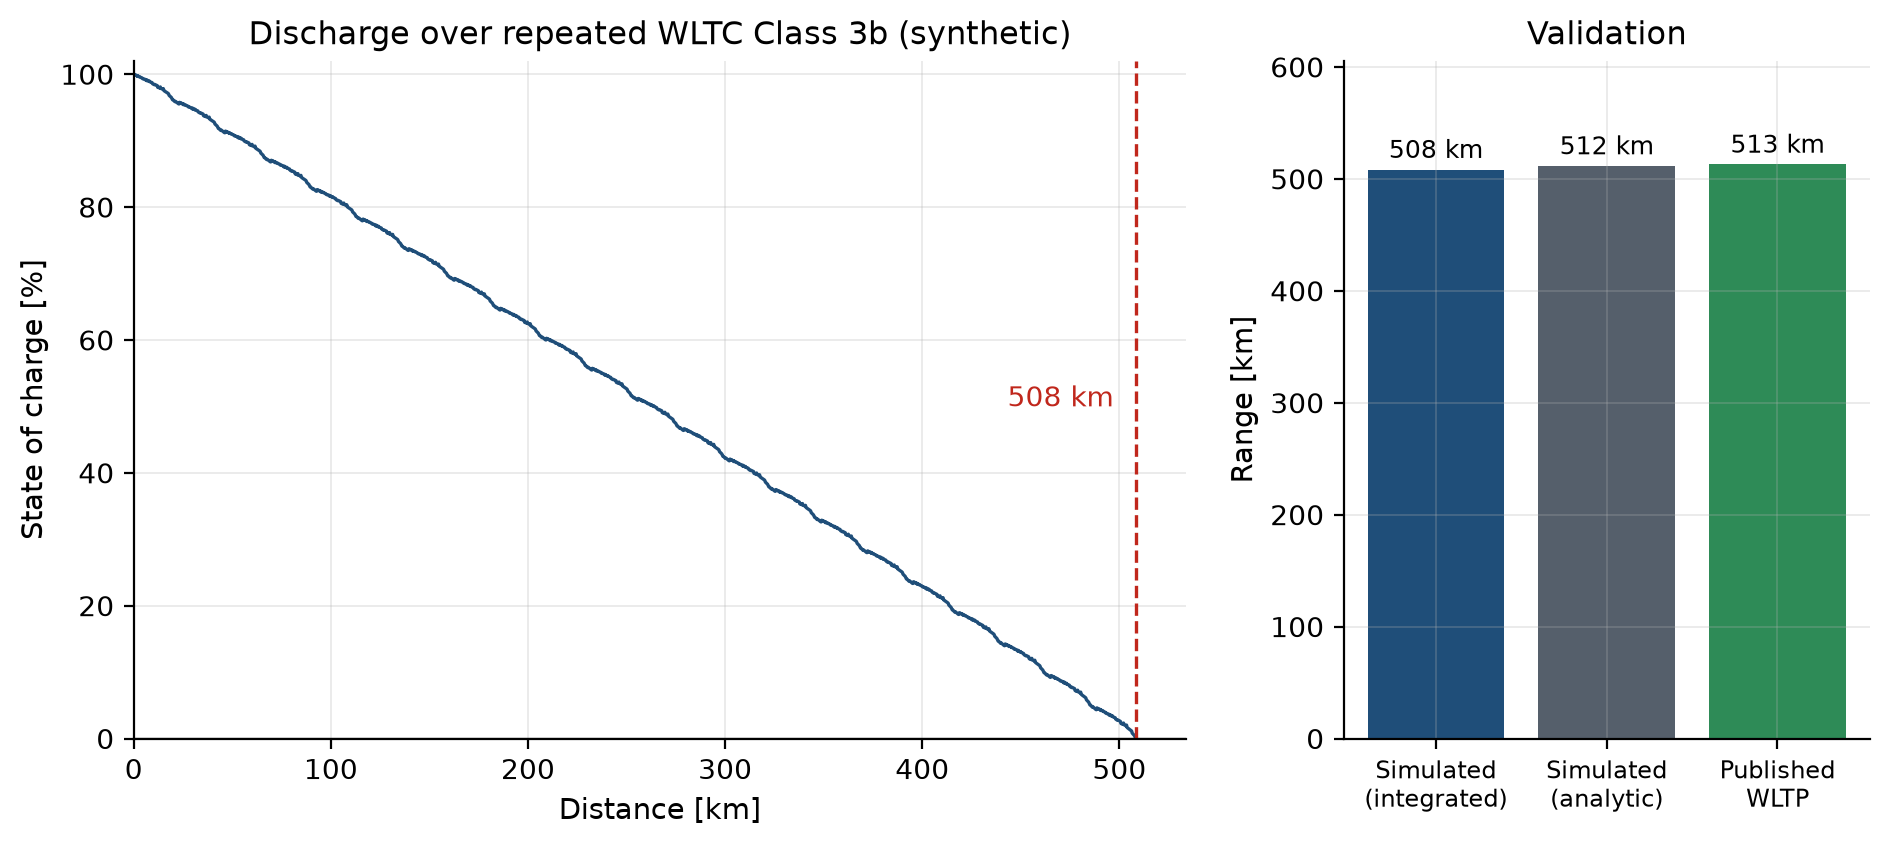
\includegraphics[width=\columnwidth]{08_range.png}
    \caption{State of charge against distance over repeated cycles to an empty
    battery, and comparison of both methods against the published figure.}
    \label{fig:range}
\end{figure}

\subsection{Range at Constant Speed}

Figure~\ref{fig:cruise} shows range and consumption at steady cruising speed,
a classic electric-vehicle characteristic. The curve has an interior maximum
because the constant auxiliary load dominates at low speed, where little
distance is covered per unit time, while aerodynamic drag dominates at high
speed. The predicted optimum lies near \SI{32}{\kilo\metre\per\hour}.

This curve is also an independent validation, discussed in the next section,
because none of its points was used in any calibration.

\begin{figure}[H]
    \centering
    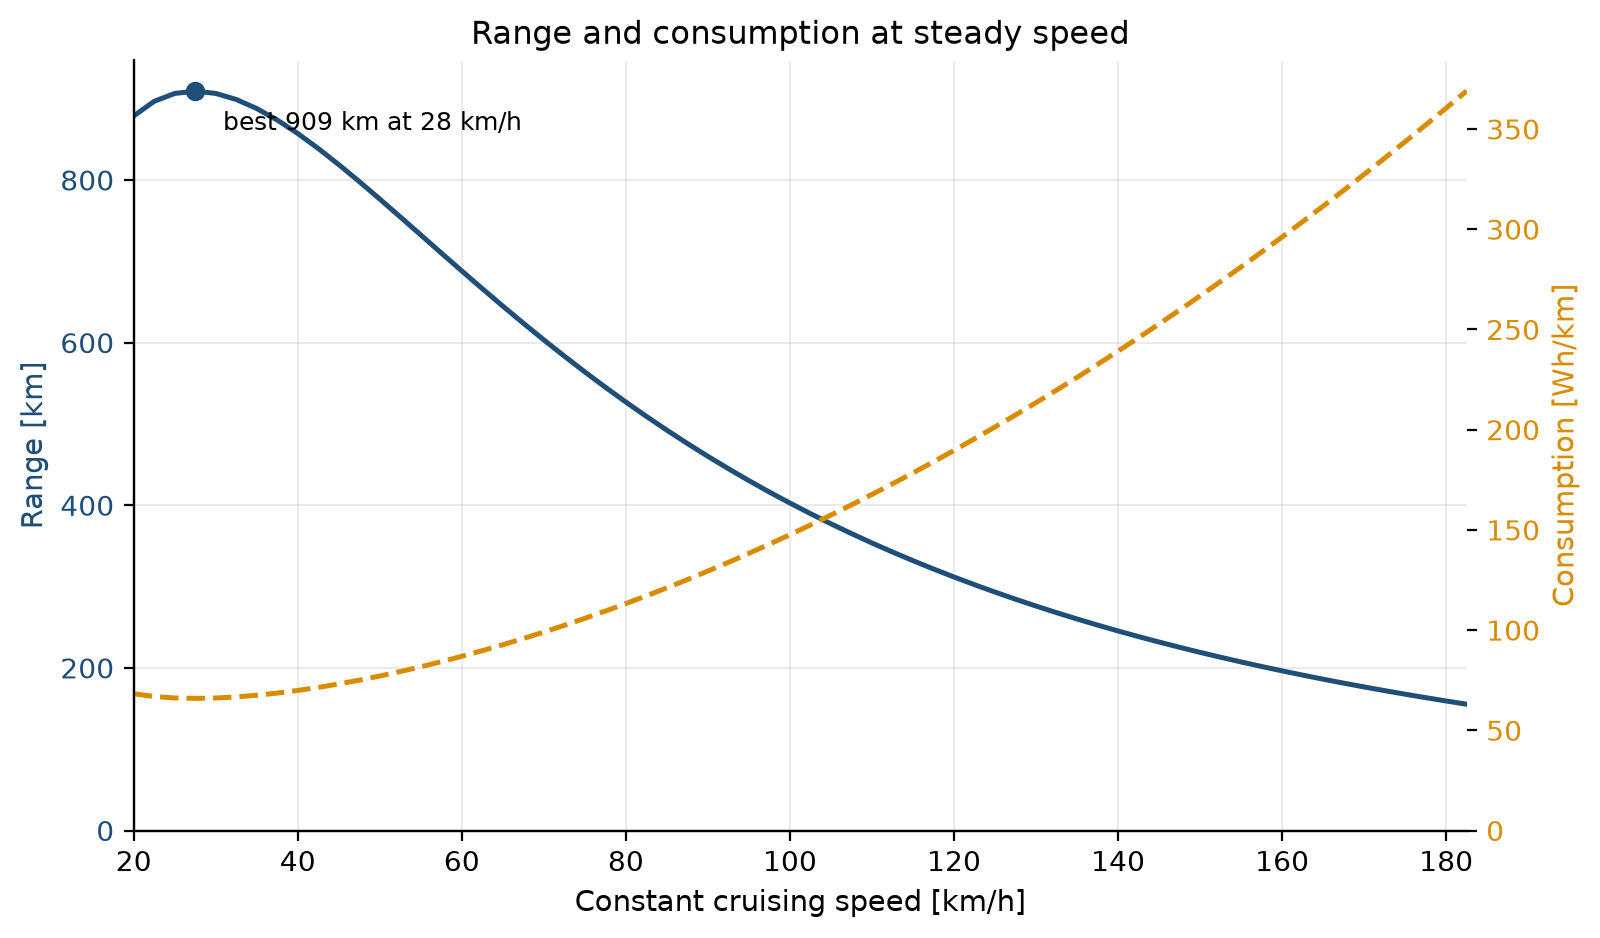
\includegraphics[width=\columnwidth]{09_constant_speed_range.png}
    \caption{Range and consumption at steady cruising speed. The interior
    maximum arises from the competition between the constant auxiliary load and
    aerodynamic drag.}
    \label{fig:cruise}
\end{figure}

\section{Validation}
\label{sec:validation}

\subsection{Against Published Figures}

Table~\ref{tab:validation} compares the model against the three figures the
manufacturer publishes. None of them was used to calibrate it, and all three
are reproduced from a single parameter set.

\begin{table}[H]
\centering
\caption{Validation against published manufacturer data. No published figure
was used as a model input.}
\label{tab:validation}
\footnotesize
\begin{tabular}{@{}lrrrr@{}}
\toprule
\textbf{Quantity} & \textbf{Sim.} & \textbf{Pub.} & \textbf{Dev.} & \textbf{Tol.} \\
\midrule
0--100 km/h (s)            & 6.14   & 6.10   & $+0.68$\,\% & $\pm10$\,\% \\
Top speed (km/h)           & 201.0  & 201.0  & $+0.00$\,\% & $\pm5$\,\%  \\
WLTP range (km)            & 508.3  & 513.0  & $-0.92$\,\% & $\pm10$\,\% \\
Consumption (kWh/100 km)   & 11.45  & 11.70  & $-2.08$\,\% & $\pm10$\,\% \\
\bottomrule
\end{tabular}
\end{table}

\subsection{Independent Checks}

Three further checks were applied that use no manufacturer data at all.

\emph{Steady-cruise consumption.} The model predicts
\SI{148}{\Whpkm} at \SI{100}{\kilo\metre\per\hour} and
\SI{213}{\Whpkm} at \SI{130}{\kilo\metre\per\hour}. Reported
real-world measurements for this vehicle fall in the ranges 140 to 150 and
190 to \SI{210}{\Whpkm} respectively~\cite{alqahtani2021}. Neither point
entered any calibration.

\emph{Energy conservation at the wheel.} Integrating Newton's second law
against speed over a cycle that starts and ends at rest requires the net wheel
work to equal the road-load dissipation plus the friction-brake dissipation.
The residual is \SI{9e-10}{\joule}.

\emph{Closure of the battery energy balance.} The four expenditure terms of
Table~\ref{tab:energy} close against the net battery energy to
\SI{1e-7}{\joule}, and the loop accumulators agree with the integral of the
battery power trace to the same tolerance under every limiting condition
tested.

\subsection{Effect of the Driving Profile}

Run over the NEDC instead, the same vehicle returns
\SI{10.90}{\kWhph} and
\SI{541}{\kilo\metre}, which is \SI{6.4}{\percent} further than on the WLTC.
The older cycle is gentler in both speed and acceleration content and therefore
flatters the vehicle, which is precisely the reason it was replaced.

\section{Assumptions and Sensitivity}
\label{sec:sensitivity}

\subsection{Rationale}

Thirty-two of the forty-nine parameters are estimates. Listing them, as
Table~\ref{tab:params} does, is necessary but not sufficient. What matters for
the credibility of the result is how much each one moves the answer.

Table~\ref{tab:tornado} varies each parameter across the interval a reasonable
engineer would call plausible and reports the resulting span in predicted
range. Figure~\ref{fig:tornado} shows the same information as a tornado chart.

An important subtlety is that the set of parameters which influence the result
depends on which road-load formulation is active. Under the coastdown form of
Equation~\ref{eq:coastdown} the wind-tunnel drag coefficient, the frontal area
and the tyre rolling-resistance coefficient influence nothing at all. A
sensitivity study that varied them regardless would place silent zeros on the
chart, which would look convincing and mean nothing. The case list is therefore
built from the active model.

\begin{table}[H]
\centering
\caption{Sensitivity of the predicted range to each assumed parameter, ranked
by influence.}
\label{tab:tornado}
\footnotesize
\begin{tabular}{@{}llrr@{}}
\toprule
\textbf{Parameter} & \textbf{Interval} & \textbf{Span} & \textbf{Of base} \\
 & & km & \% \\
\midrule
HVAC load            & 0--3000 W          & 181 & 35.6 \\
Regen power limit    & 0--90 kW           & 115 & 22.6 \\
Battery capacity     & 57.5--66 kWh       &  70 & 13.7 \\
Coastdown $F_2$      & 0.340--0.440       &  52 & 10.1 \\
Coastdown $F_0$      & 95--140 N          &  52 & 10.1 \\
Payload              & 0--400 kg          &  40 &  7.9 \\
Coastdown $F_1$      & 1.30--2.45         &  28 &  5.6 \\
Gear efficiency      & 0.960--0.992       &  25 &  4.8 \\
Motor windage $k_w$  & 1.0--3.0\,e--6     &  22 &  4.3 \\
\bottomrule
\end{tabular}
\end{table}

\subsection{Basis of the Dominant Assumptions}

Because the ranking in Table~\ref{tab:tornado} identifies which estimates
carry the result, the basis of the five most influential is stated explicitly
in Table~\ref{tab:basis}. The remaining assumptions are documented in the same
form in the machine-readable parameter file.

\begin{table}[H]
\centering
\caption{Basis for the five assumptions that most influence the predicted
range. All values are \asm{estimates}.}
\label{tab:basis}
\footnotesize
\begin{tabular}{@{}>{\raggedright\arraybackslash}p{0.26\columnwidth}>{\raggedright\arraybackslash}p{0.62\columnwidth}@{}}
\toprule
\textbf{Assumption} & \textbf{Basis} \\
\midrule
HVAC load \asm{0--3000 W} &
Certification is run with auxiliaries off. The upper bound corresponds to
cabin and battery heating at \SI{0}{\celsius}, consistent with published
cold-weather consumption studies~\cite{iora2019}. \\
\addlinespace
Regen power limit \asm{\SI{70}{\kilo\watt}} &
Observed regeneration ceiling on single-motor variants. The lower bound of the
interval represents friction braking only. \\
\addlinespace
Gross capacity \asm{\SI{62.5}{\kilo\watt\hour}} &
Not published. Taken from independent pack teardowns and battery-management
logs for the LFP pack; the interval spans the range those sources report. \\
\addlinespace
Coastdown $F_0$, $F_1$, $F_2$ &
Converted to SI from published certification coastdown targets. The intervals
reflect the variation with wheel size, tyre specification and model
year~\cite{epacoastdown}. \\
\addlinespace
Loss coefficients $k_c$, $k_i$, $k_w$, $P_0$ &
Fitted by least squares to seven operating points representative of a
liquid-cooled automotive permanent-magnet drive unit~\cite{larminie2012,
sarlioglu2017}. \\
\bottomrule
\end{tabular}
\end{table}

\subsection{Interpretation}

The ranking is itself a result. The auxiliary load dominates, worth
\SI{35.6}{\percent} of the baseline range on its own, and it is the one
quantity in the list that the driver actually controls. The regeneration power
limit follows, at \SI{22.6}{\percent}.

The drivetrain assumptions, which were the hardest to pin down and which
required the loss-model fit described in Section~\ref{sec:model}, matter least:
gear efficiency and motor windage together account for under
\SI{10}{\percent}. This is the reassuring outcome. The answer does not rest on
the values that were estimated with the least confidence.

\begin{figure}[H]
    \centering
    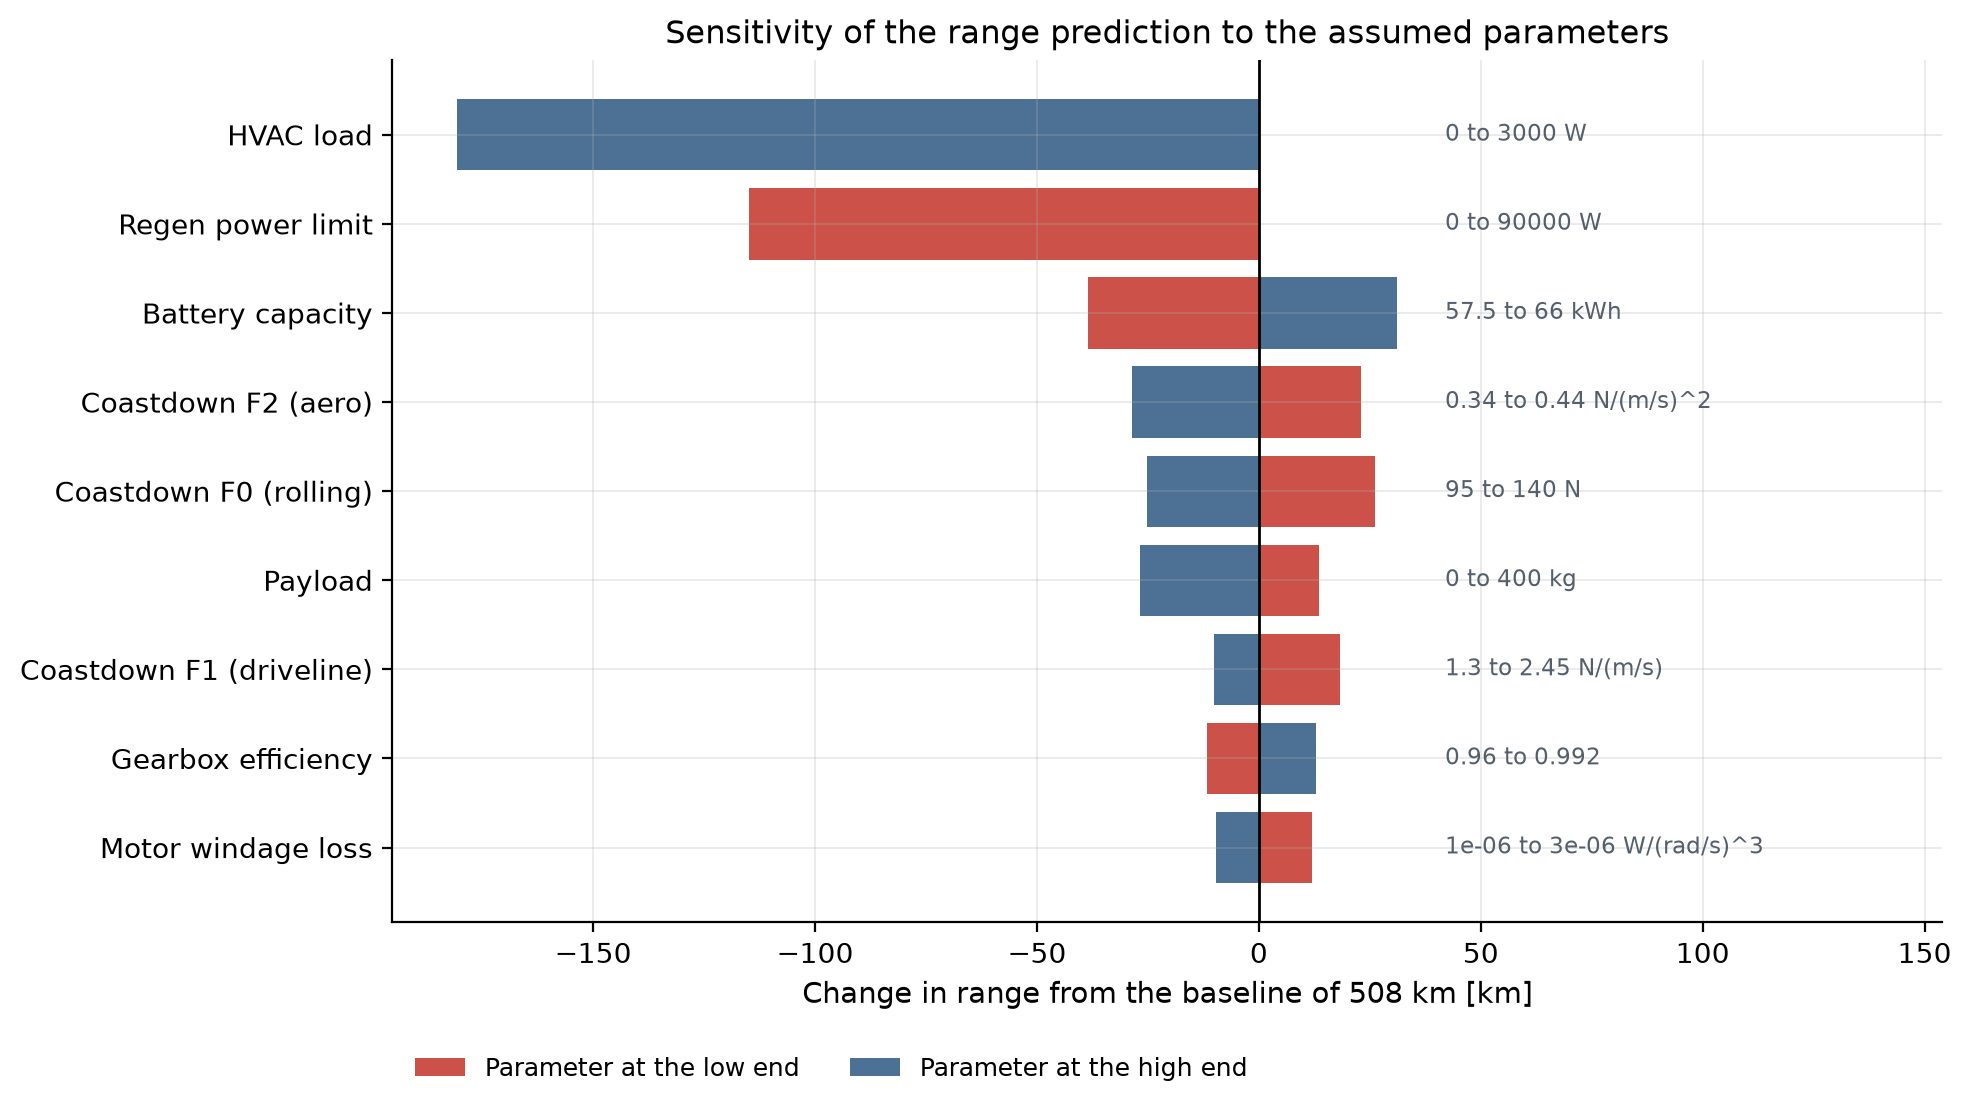
\includegraphics[width=\columnwidth]{10_sensitivity_tornado.png}
    \caption{Sensitivity of the predicted range to each assumed parameter
    across its plausible interval.}
    \label{fig:tornado}
\end{figure}

\section{Real-World Conditions}
\label{sec:scenarios}

The certification figure is measured with the auxiliaries switched off, a
defined test mass and standard air. Real driving is none of those
things~\cite{iora2019}. Table~\ref{tab:scenarios} and
Figure~\ref{fig:scenarios} give the predicted range under five named
conditions, all evaluated on the same cycle and differing only in the
parameters a driver or the weather changes.

The spread between the certification case and a winter morning with cabin and
battery heating is \SI{215}{\kilo\metre}, or \SI{42}{\percent}. A driver told
to expect \SI{508}{\kilo\metre} and finding \SI{293}{\kilo\metre} has not been
misled by a faulty vehicle; they have encountered the difference between a
standardised test and the world.

\begin{table}[H]
\centering
\caption{Predicted range under real-world conditions, all on the WLTC cycle.}
\label{tab:scenarios}
\footnotesize
\begin{tabular}{@{}llrr@{}}
\toprule
\textbf{Scenario} & \textbf{Conditions} & \textbf{Range} & \textbf{$\Delta$} \\
 & & km & \% \\
\midrule
WLTP certification  & Aux.\ off, driver only    & 508 & --- \\
Mild weather        & Ventilation, 2 occupants  & 455 & $-10$ \\
Loaded, roof box    & 5 occupants plus luggage  & 394 & $-22$ \\
Summer, A/C         & \SI{30}{\celsius} ambient & 378 & $-26$ \\
Winter, heating     & \SI{0}{\celsius}, cold tyres & 293 & $-42$ \\
\bottomrule
\end{tabular}
\end{table}

\begin{figure}[H]
    \centering
    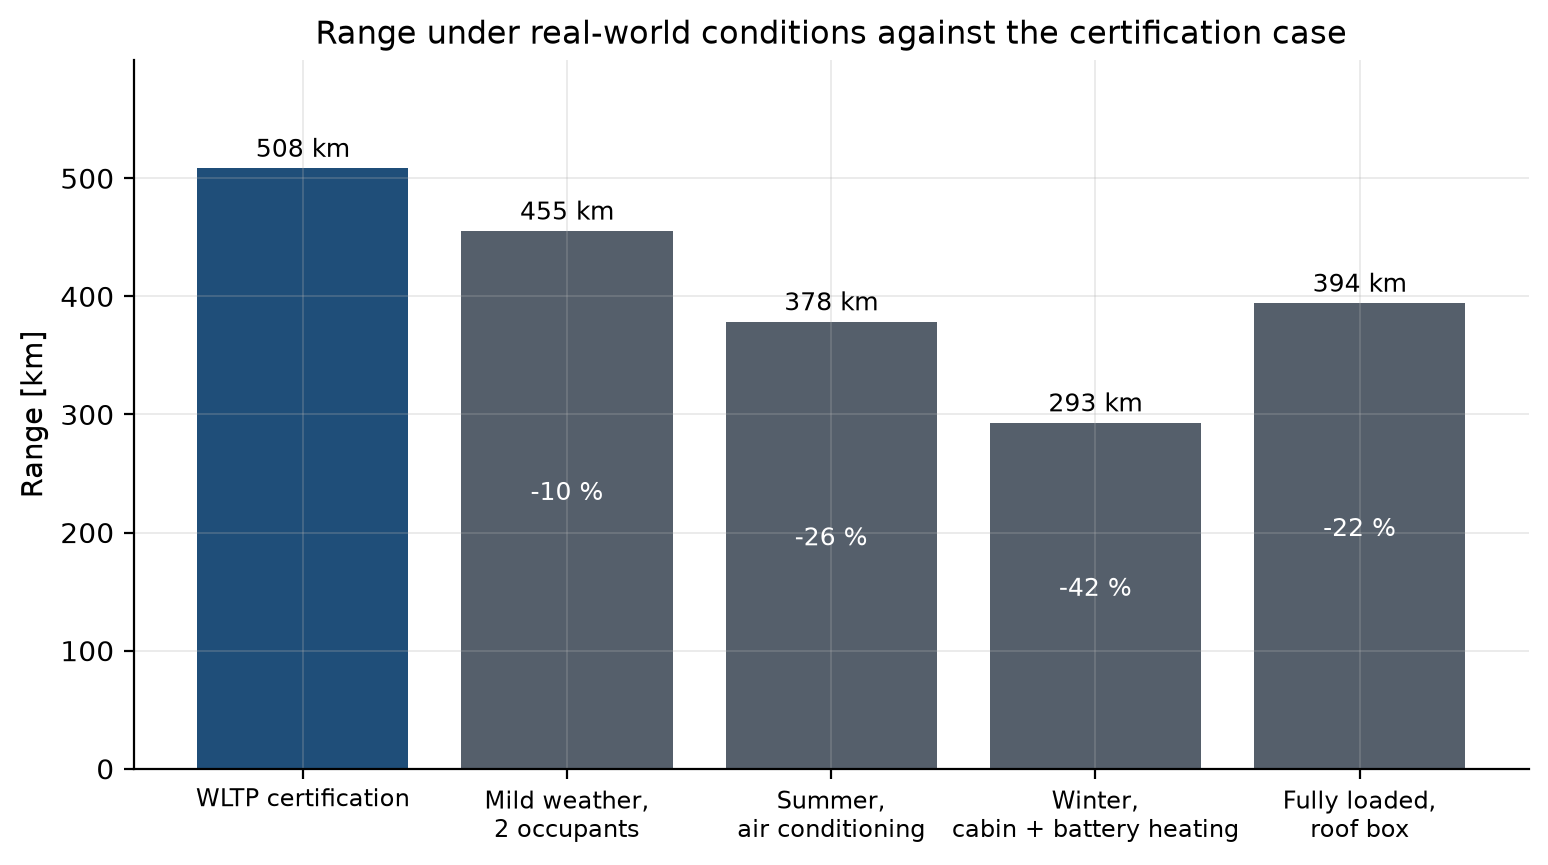
\includegraphics[width=\columnwidth]{11_scenarios.png}
    \caption{Predicted range under real-world conditions against the
    certification case.}
    \label{fig:scenarios}
\end{figure}

\section{Software Implementation}
\label{sec:software}

\subsection{Structure}

The model is implemented as an installable Python package of fifteen modules,
built on NumPy~\cite{harris2020numpy}, SciPy~\cite{virtanen2020scipy} and
Matplotlib~\cite{hunter2007matplotlib}. Responsibilities are separated by
physical subsystem: parameter loading and the assumption register, road load,
powertrain, battery, performance characteristics, driving cycles, the cycle
simulator, range calculation, the sensitivity study, plotting, and report
generation.

All internal computation is in SI units, with conversion confined to the
input and output boundaries. Every parameter is loaded from a single versioned
YAML file in which each entry carries its numeric value, its unit, a provenance
string, and a boolean flag recording whether it is an assumption. The red
marking in this report is generated from that flag rather than applied by hand,
so it cannot fall out of step with the model.

\subsection{Reproducibility and Verification}

A single command regenerates every figure, table and document in this report
from the parameter file alone, taking approximately \SI{80}{\second}. The
numbers quoted in the text are produced by the same run that produces the
figures, so they cannot diverge.

The package is accompanied by 125 automated tests, which execute in about
\SI{76}{\second}. They check each road-load term against an independent hand
calculation rather than against the code's own output; verify that the motor
envelope corner point, the constant-power region and the peak efficiency fall
in physically plausible bands; confirm that a slow full discharge returns the
nameplate energy and that the current solution satisfies
Equation~\ref{eq:current}; compare both driving cycles against their published
statistics phase by phase; and assert the acceptance criteria stated in
Section~\ref{sec:validation}.

Two tests deserve specific mention because they guard against failures that
would otherwise be invisible. One drives an artificially underpowered vehicle
over the cycle and asserts that the simulator flags the steps it cannot follow
rather than silently reporting an impossible result. The other asserts that no
sensitivity case is inert, which guards the trap described in
Section~\ref{sec:sensitivity}.

\section{Limitations}
\label{sec:limitations}

Four limitations bound the applicability of these results.

\emph{No thermal model.} Continuous-power derating and the rise in battery
internal resistance at low temperature are not represented. Neither binds on a
legislative cycle, whose power demands are modest and brief, but both matter
for sustained high-power driving and for cold starts.

\emph{No battery ageing.} The results describe a new vehicle. Capacity fade and
resistance growth over the life of the pack are outside the scope.

\emph{Fitted rather than measured efficiency.} The drive-unit efficiency comes
from the four-term loss model of Equation~\ref{eq:loss} fitted to plausible
operating points, not from a measured map. The sensitivity study shows this
contributes under \SI{5}{\percent} to the range prediction.

\emph{Longitudinal dynamics only.} Lateral dynamics, suspension behaviour and
the tyre slip that accompanies real cornering are not modelled, nor is charging
behaviour or interaction with the grid.

\section{Conclusions}

A longitudinal model of the Tesla Model~3 RWD reproduces all three published
performance figures from a single parameter set, with no figure tuned
individually: acceleration to \SI{100}{\kilo\metre\per\hour} within
\SI{0.7}{\percent}, top speed exactly, and WLTP range within
\SI{0.9}{\percent}. Steady-cruise consumption, which entered no calibration,
falls inside the measured real-world band at both \SI{100}{} and
\SI{130}{\kilo\metre\per\hour}.

Three findings are worth carrying forward.

\textbf{The vehicle is traction-limited off the line, not torque-limited.} The
rear tyres, not the machine, set the acceleration for roughly the first third
of the run to \SI{100}{\kilo\metre\per\hour}. A model without dynamic
axle-load transfer is optimistic by about \SI{15}{\percent}.

\textbf{Top speed is a software decision.} The electronic limiter binds well
below both the machine's mechanical speed ceiling and the point at which drag
would overcome the available tractive force.

\textbf{The advertised drag coefficient does not predict range.} The
coastdown-derived drag area exceeds the wind-tunnel figure by
\SI{29}{\percent}, because a wind tunnel excludes wheel rotation and cooling
airflow. Both numbers are correct, but only one of them predicts energy, and
using the textbook decomposition alone under-predicts road load by 15 to
\SI{19}{\percent} above \SI{80}{\kilo\metre\per\hour}.

Finally, the sensitivity study shows that a result built on thirty-two
estimated parameters can still be defensible, provided the estimates that
dominate are identified. Here the auxiliary load dominates and the drivetrain
assumptions do not, which means the prediction does not rest on the quantities
that were hardest to determine.

\section*{Acknowledgments}

\subsection*{Author Contributions}
All authors contributed to the formulation of the vehicle model, the selection
and justification of the assumed parameters, the interpretation of the
sensitivity study, and the preparation of this manuscript. The software
implementation, the validation campaign and the figure generation were carried
out collaboratively. The authors thank the teaching staff of the
\emph{Electric Vehicle Technologies and Applications} module for guidance on
vehicle longitudinal dynamics and legislative test procedures.

\subsection*{Funding}
This work was supported by the Department of Control, Computer and
Communications Engineering at THM University of Applied Sciences.

\subsection*{Conflicts of Interest}
The authors declare no conflicts of interest regarding the publication of this
article.

\subsection*{Data Availability}
\begin{sloppypar}
All source code, the vehicle parameter file with the provenance of every value,
the generated assumption register, and the scripts that regenerate every figure
and table in this report are available in the open-source repository:
\url{https://github.com/tarikbilla/Electric-Vehicle-Technologies-and-Applications}.
\end{sloppypar}

\section*{References}
\nocite{*}
\printbibliography[heading=none]
\end{document}
